\documentclass[fr,license=none]{../../../eplsummary}
\usepackage{../../../eplcommon}
\usepackage{graphicx}
\usepackage{mathenv}
\usepackage{multicol}
\usepackage{multirow}
\usepackage{subcaption}
\usepackage{wrapfig}
\usepackage{eurosym}
\usepackage{framed}
\usepackage{enumitem}
\usepackage{color}
\usepackage{xcolor}
\usepackage{titling}
\usepackage{float}
\usepackage{empheq}
\definecolor{violet}{RGB}{118,57,222}
\definecolor{violet2}{RGB}{110,5,247}
\definecolor{mauvedef}{RGB}{57,0,114}
\definecolor{miorangerouge}{RGB}{215,64,0}
\definecolor{vert}{RGB}{0,121,16}
\graphicspath{{img/}}
\newcommand*\widefbox[1]{\fbox{\hspace{2em}#1\hspace{2em}}}
\newcommand{\elasticity}{\varepsilon}
\newcommand{\pcompt}{\pi}
\newcommand{\ppur}{\pi_{\textnormal{pur}}}
\newcommand{\surplus}{s}
\newcommand{\surpluscons}{S_{\textnormal{c}}}
\newcommand{\surplusprod}{S_{\textnormal{p}}}
\newcommand{\qi}{q_i}
\newcommand{\surpluscoll}{S}
\newcommand{\Lagr}{\mathcal{L}}
\newcommand{\cmarg}{C_{\textnormal{m}}}
\newcommand{\rmarg}{R_{\textnormal{m}}}
\newcommand{\cmoy}{C_{\textnormal{M}}}
\newcommand{\rmoy}{R_{\textnormal{M}}}
\newcommand{\cvar}{C_{\textnormal{V}}}
\newcommand{\cfixe}{C_{\textnormal{F}}}
\newcommand{\cmoyvar}{C_{\textnormal{MV}}}
\newcommand{\cmoyfixe}{C_{\textnormal{MF}}}
\newcommand{\popt}{p^*}
\newcommand{\qopt}{q^*}
\newcommand{\mathsc}[1]{{\normalfont\textsc{#1}}}
\newcommand{\pmon}{p_{\mathsc{mon}}}
\newcommand{\qmon}{q_{\mathsc{mon}}}
\newcommand{\pimon}{\pcompt_{\mathsc{mon}}}
\newcommand{\scmon}{\surpluscons^{\mathsc{mon}}}
\newcommand{\sccp}{\surpluscons^{\mathsc{cp}}}
\usepackage{interval}
\usepackage{bm}


% TODO : add this to eplmath and replace with a usepackage, and remove the one in the stat-fsab1105 package.

\makeatletter
\let\save@mathaccent\mathaccent
\newcommand*\if@single[3]{%
	\setbox0\hbox{${\mathaccent"0362{#1}}^H$}%
	\setbox2\hbox{${\mathaccent"0362{\kern0pt#1}}^H$}%
	\ifdim\ht0=\ht2 #3\else #2\fi
}
%The bar will be moved to the right by a half of \macc@kerna, which is computed by amsmath:
\newcommand*\rel@kern[1]{\kern#1\dimexpr\macc@kerna}
%If there's a superscript following the bar, then no negative kern may follow the bar;
%an additional {} makes sure that the superscript is high enough in this case:
\newcommand*\widebar[1]{\@ifnextchar^{{\wide@bar{#1}{0}}}{\wide@bar{#1}{1}}}
%Use a separate algorithm for single symbols:
\newcommand*\wide@bar[2]{\if@single{#1}{\wide@bar@{#1}{#2}{1}}{\wide@bar@{#1}{#2}{2}}}
\newcommand*\wide@bar@[3]{%
	\begingroup
	\def\mathaccent##1##2{%
		%Enable nesting of accents:
		\let\mathaccent\save@mathaccent
		%If there's more than a single symbol, use the first character instead (see below):
		\if#32 \let\macc@nucleus\first@char \fi
		%Determine the italic correction:
		\setbox\z@\hbox{$\macc@style{\macc@nucleus}_{}$}%
		\setbox\tw@\hbox{$\macc@style{\macc@nucleus}{}_{}$}%
		\dimen@\wd\tw@
		\advance\dimen@-\wd\z@
		%Now \dimen@ is the italic correction of the symbol.
		\divide\dimen@ 3
		\@tempdima\wd\tw@
		\advance\@tempdima-\scriptspace
		%Now \@tempdima is the width of the symbol.
		\divide\@tempdima 10
		\advance\dimen@-\@tempdima
		%Now \dimen@ = (italic correction / 3) - (Breite / 10)
		\ifdim\dimen@>\z@ \dimen@0pt\fi
		%The bar will be shortened in the case \dimen@<0 !
		\rel@kern{0.6}\kern-\dimen@
		\if#31
		\overline{\rel@kern{-0.6}\kern\dimen@\macc@nucleus\rel@kern{0.4}\kern\dimen@}%
		\advance\dimen@0.4\dimexpr\macc@kerna
		%Place the combined final kern (-\dimen@) if it is >0 or if a superscript follows:
		\let\final@kern#2%
		\ifdim\dimen@<\z@ \let\final@kern1\fi
		\if\final@kern1 \kern-\dimen@\fi
		\else
		\overline{\rel@kern{-0.6}\kern\dimen@#1}%
		\fi
	}%
	\macc@depth\@ne
	\let\math@bgroup\@empty \let\math@egroup\macc@set@skewchar
	\mathsurround\z@ \frozen@everymath{\mathgroup\macc@group\relax}%
	\macc@set@skewchar\relax
	\let\mathaccentV\macc@nested@a
	%The following initialises \macc@kerna and calls \mathaccent:
	\if#31
	\macc@nested@a\relax111{#1}%
	\else
	%If the argument consists of more than one symbol, and if the first token is
	%a letter, use that letter for the computations:
	\def\gobble@till@marker##1\endmarker{}%
	\futurelet\first@char\gobble@till@marker#1\endmarker
	\ifcat\noexpand\first@char A\else
	\def\first@char{}%
	\fi
	\macc@nested@a\relax111{\first@char}%
	\fi
	\endgroup
}
\makeatother


\hypertitle{Sciences humaines - Économie de l'entreprise}{4}{FSAB}{1803}
{Eve Leroy\and Gilles Peiffer}
{Jacqueline Boucher et Julien Hendrickx}

\section{Marché de concurrence parfaite} % 1


	\begin{mydef}[\textcolor{violet2}{\underline{Capital}} (\textcolor{miorangerouge}{K})]
		Patrimoine possédé par un individu, une famille ou une entreprise
		et pouvant rapporter un revenu.
	\end{mydef}
	\bigbreak


	\begin{mydef}[\textcolor{violet2}{\underline{Économie}}]
		Ensemble des stratégies humaines mises en \oe{}uvre
		pour assurer la meilleure utilisation (optimisation) possible de ressources rares.

		\begin{myrem}
			Si les ressources n'étaient pas rares,
			la question de meilleure utilisation ne se poserait pas.
			La rareté des ressources peut évoluer dans le temps.
		\end{myrem}
	\end{mydef}
	\bigbreak



	\begin{mydef}[\textcolor{violet2}{\underline{Entreprise}}]
		Une entreprise fait deux choses:
		\begin{itemize}[label={\color{violet} \textbullet}]
			\item investir pour dégager un profit (holdings, particuliers);
			\item organiser (administrations,\dots).
		\end{itemize}

		\begin{figure}[H]
			\centering
			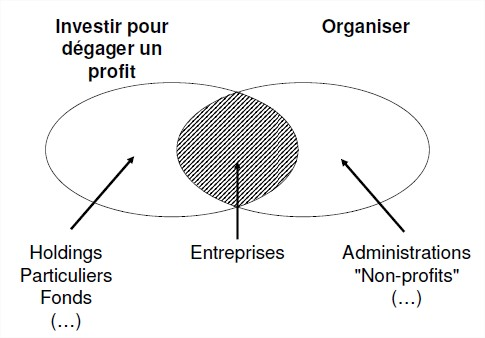
\includegraphics[scale=0.5]{Entreprise1.jpg}
			\caption{Buts d'une entreprise.}
			\label{fig:firm_goals}
		\end{figure}
	\end{mydef}
	\bigbreak




	\begin{mydef}[\textcolor{violet2}{\underline{Investissement}}]
		Opération qui permet de renouveler
		et d'accroître le capital d'une économie.
	\end{mydef}
	\bigbreak


	\begin{mydef}[\textcolor{violet2}{\underline{Holding}}]
		Groupe de gens qui ont de l'argent
		et qui investissent dans les entreprises.
	\end{mydef}
	\bigbreak



	\renewcommand{\arraystretch}{1.5} % Espacement dans les cellules = 150% de l'espacement normal pour 1.5
	\begin{center}
		\begin{tabular}{p{0.45\textwidth}p{0.45\textwidth}} %\raggedleft, \raggedright et \centering puis plus \\ mais \tabularnewline
			\hline
			\centering{\textcolor{violet2}{\textbf{Microéconomie}}} & \centering{\textcolor{violet2}{\textbf{Macroéconomie}}} \tabularnewline
			Partie de l'économie qui étudie les comportements des agents individuels (consommateurs, producteurs,\dots)
			&
			Partie de l'économie qui étudie les comportements des grands agrégats des économies nationales, européennes ou internationales
			(PNB, croissance, emploi, inflation, devises,\dots)
			\bigbreak

			\centering{$\implies$ Plus général}\tabularnewline
			 &\\
			Applications: tarification, choix d'investissements, économie industrielle, structure des entreprises, concurrence,\dots
			&
			Applications: politiques économiques et sociales (monnaies, budgets, relances, taux d'intérêt,\dots)\\
			\centering{Ingénieur = Acteur} & \centering{Ingénieur = Sujet}\tabularnewline
			\centering{Formation} & \centering{Information}\tabularnewline
			\hline
		\end{tabular}
	\end{center}
	\bigbreak



	\begin{mydef}[\textcolor{violet2}{\underline{Modes d'approche}}]
		Il y a différents modes d'approche:
		\begin{itemize}[label={\color{violet} \textbullet}]
			\item \textbf{agent} ( = acteur) : consommateurs, travailleurs, entreprises,\dots{} (économie de la consommation);
			\item \textbf{domaine} : énergie, banque, assurance, environnement, santé,\dots{}
		\end{itemize}
	\end{mydef}
	\bigbreak



	\begin{mydef}[\textcolor{violet2}{\underline{Travail}} (\textcolor{miorangerouge}{L})]
		Activité professionnelle régulière et rémunérée.
		\begin{myrem}
			L vient de Labor.
		\end{myrem}
	\end{mydef}
	\bigbreak


	\begin{mydef}[\textcolor{violet2}{\underline{Variable active}}]
		Deux caractéristiques des variables actives sont:
		\begin{itemize}[label={\color{violet} \textbullet}]
			\item variable qui change si on l'observe ou si on la mesure;
			\item mesures moins précises.
		\end{itemize}
	\end{mydef}
	\bigbreak


	\begin{mydef}[\textcolor{violet2}{\underline{Variable passive}}]
		Deux caractéristiques des variables actives sont:
		\begin{itemize}[label={\color{violet} \textbullet}]
			\item variable qui ne change pas si on l'observe ou non;
			\item mesures précises.
		\end{itemize}
	\end{mydef}
	\bigbreak


	%%%%%%%%%%%%%%%%%%%%%%%%%%%%%%%%%%%%%%%%%%%%%%%%%%%%%%%%%%%%%%%%%%%%%%%%%%%%%%%%%

	\subsection{Notion de ``marché''} % 1.1

		\begin{mydef}[\textcolor{violet2}{\underline{Marché}}]
			Un marché a les caractéristiques suivantes:
			\begin{itemize}[label={\color{violet} \textbullet}]
				\item groupe d'individus et d'entreprises;
				\item en relation les uns avec les autres (quand deux partis s'accordent sur un échange);
				\item pour acheter ou vendre des biens (ou des services). \begin{myexem}
					Troc,\dots;
				\end{myexem}
				\item étranger à toute contrainte de force ou de morale
				(les deux partis sont libres).
				\begin{myexem}
					Achat d'organes, système féodal (pas de libertés),\dots;
				\end{myexem}
				\item échange de marché immédiatement libératoire.
				Il ne s'agit donc pas d'une économie du don
				(aide apportée pour quelque chose, attend un contre-don).
			\end{itemize}
			Il
			\begin{itemize}[label={\color{violet} \textbullet}]
				\item \textbf{est caractérisé par}
				(en fonction des mécanismes de concurrence qui régissent le marché):
				\begin{itemize}[label={\color{Orchid} \textbullet}]
					\item le volume de transactions;
					\item le prix,
				\end{itemize}
				\item \textbf{dépend de}:
				\begin{itemize}[label={\color{Orchid} \textbullet}]
					\item la nature des biens échangés;
					\item le lieu de l'échange;
					\item le temps de l'échange.
				\end{itemize}
			\end{itemize}
			Il confronte l'offre et la demande (pour 1 seul marché)
			et conduit à la détermination d'un prix.
		\end{mydef}
		\bigbreak



	%%%%%%%%%%%%%%%%%%%%%%%%%%%%%%%%%%%%%%%%%%%%%%%%%%%%%%%%%%%%%%%%%%%%%%%%%%%%%%%%%

	\subsection{Équilibre du marché} % 1.2

		\begin{mydef}[\textcolor{violet2}{\underline{Équilibre de marché}}]
			Il est défini à l'intersection des courbes d'offre et de demande
			et il fixe un prix \textcolor{miorangerouge}{$\popt $}
			pour une quantité échangée \textcolor{miorangerouge}{$\qopt $}. Généralement, $D(p)$ est \textcolor{red}{décroissante}
			et $O(p)$ est \textcolor{vert}{croissante}.

			\begin{figure}[H]
				\centering
				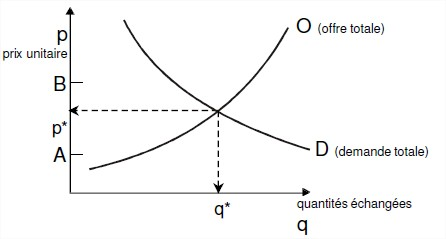
\includegraphics[scale=0.5]{EquilibreMarche.jpg}
				\caption{L'équilibre de marché est l'intersection
				entre la courbe d'offre et de la courbe de demande.}
				\label{fig:market_equilibrium}
			\end{figure}
		\end{mydef}

		\begin{mydef}[\textcolor{violet2}{\underline{Équilibre}}]
			L'équilibre en économie est un processus d'ajustement progressif :
			\begin{empheq}[box=\widefbox]{alignat*=2}
			\tag{}
				&\textnormal{Si } p < \popt , \: O < D &&\textnormal{ et } p  \: \textcolor{vert}{\nearrow} \\
				\tag{}
				&\textnormal{Si } p > \popt , \: O > D &&\textnormal{ et } p  \: \textcolor{red}{\searrow}
			\end{empheq}
		\end{mydef}
		\bigbreak


	%%%%%%%%%%%%%%%%%%%%%%%%%%%%%%%%%%%%%%%%%%%%%%%%%%%%%%%%%%%%%%%%%%%%%%%%%%%%%%%%%

	\subsection{Fonctions d'offre et de demande} % 1.3

		\begin{mydef}[\textcolor{violet2}{\underline{Demande}}]
			\begin{figure}[H]
				\centering
				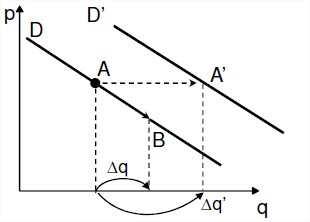
\includegraphics[scale=0.5]{1-2Demande.jpg}
				\caption{}\label{fig:demand}
			\end{figure}

			\begin{itemize}[label={\color{violet} \textbullet}]
				Sur la \figuref{demand},
				\item le \textbf{déplacement AB} est la réaction des consommateurs à une \textcolor{red}{$\searrow$} du prix du marché
				(autres paramètres constants);
				\item la \textbf{translation de la courbe}
				montre qu'à \textcolor{blue}{prix constant},
				\textcolor{miorangerouge}{$q$} demandée \textcolor{vert}{$\nearrow$}.
				Liée à d'autre facteurs que le prix
				(revenus, goûts, prix d'autres produits, fiscalité,\dots).
			\end{itemize}
		\end{mydef}
		\bigbreak


		\begin{mydef}[\textcolor{violet2}{\underline{Offre}}]

			\begin{figure}[H]
				\centering
				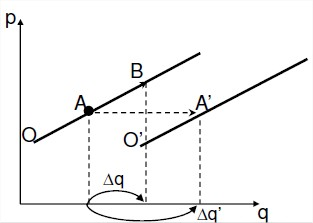
\includegraphics[scale=0.5]{1-2Offre.jpg}
				\caption{}\label{fig:supply}
			\end{figure}

			\begin{itemize}[label={\color{violet} \textbullet}]
				Sur la \figuref{supply},
				\item le \textbf{déplacement AB} montre que les quantités offertes \textcolor{vert}{$\nearrow$}
				à cause d'une \textcolor{vert}{$\nearrow$} de prix;
				\item la \textbf{translation de la courbe}
				montre qu'à \textcolor{blue}{prix constant},
				l'offre \textcolor{vert}{$\nearrow$}.
				Liée à d'autre facteurs que le prix
				(technologie, réglementation, fiscalité,\dots).
			\end{itemize}
		\end{mydef}
		\bigbreak


		\begin{mydef}[\textcolor{violet2}{\underline{Rente}}]
			Limitation dans l'offre.
		\end{mydef}
		\bigbreak



		%%%%%%%%%%%%%%%%%%%%%%%%%%%%%%%%%%%%%%%%%%%%%%%%%%%%%%%%%%%%%%%%%%%%%%%%%%%%%%%%%

	\subsection{Hypothèses fondamentales du marché de concurrence ``pur et parfait''} % 1.4


		Elles portent sur le comportement des agents économiques
		et sur le fonctionnement du marché.

		\begin{myhyp}[\textbf{Atomicité} de l'offre et de la demande]
			Infinité d'acheteurs et d'offreurs sur le marché.
			\begin{itemize}[label={\color{violet} \textbullet}]
				\item Aucun agent ne peut influencer le prix.
				\item Les agents ne se coalisent pas pour acquérir un tel pouvoir.
			\end{itemize}
		\end{myhyp}
		\bigbreak
		\begin{myhyp}[\textbf{Homogénéité} du produit]
			Un producteur ne peut pas
			différencier son produit de celui des autres.
		\end{myhyp}
		\bigbreak
		\begin{myhyp}[\textbf{Transparence} du marché]
			Tous les acteurs du marché sont informés $\implies$ information parfaite sur tous les prix,
			quantités et caractéristiques du produit.
		\end{myhyp}
		\bigbreak
		\begin{myhyp}[\textbf{Mobilité parfaite}]
			Libre entrée/sortie du marché.
		\end{myhyp}
		\bigbreak

		\begin{mydef}[\textcolor{violet2}{\underline{Price Taker}}]
			Le prix est imposé aux offreurs et demandeurs par les hypothèses du marché.
		\end{mydef}
		\bigbreak


		%%%%%%%%%%%%%%%%%%%%%%%%%%%%%%%%%%%%%%%%%%%%%%%%%%%%%%%%%%%%%%%%%%%%%%%%%%%%%%%%%

	\subsection{Utilité du modèle de concurrence parfaite} % 1.5

		Le modèle de concurrence parfaite ne reste en effet que ça:
		un modèle. Il a les caractéristiques suivantes:

		\begin{itemize}[label={\color{violet} \textbullet}]
			\item il est une \textbf{approximation} :
			certains marchés ne sont pas si éloignés que ça du modèle parfait.
			\item il est un \textbf{point de référence} :
			on peut calculer l'écart entre un marché réel et parfait.
			\item il permet de \textbf{mesurer} :
			on peut voir ce que ça donne
			quand certaines des quatre hypothèses
			ne sont plus parfaites.
		\end{itemize}
		\bigbreak


		%%%%%%%%%%%%%%%%%%%%%%%%%%%%%%%%%%%%%%%%%%%%%%%%%%%%%%%%%%%%%%%%%%%%%%%%%%%%%%%%%

	\subsection{Demande du consommateur - utilité et surplus} % 1.6


		Modèle néo-classique basé sur les maximisations
		(fin du XIX\textsuperscript{e}).
		Monde quantitatif, mathématique.
		\bigbreak


		\begin{mydef}[\textcolor{violet2}{\underline{Courbe de demande globale}}]
			La courbe de demande peut être définie de plusieurs façons:
			\begin{itemize}[label={\color{violet} \textbullet}]
				\item c'est la \textbf{dérivée de l'utilité};
				\item c'est aussi la $\sum$ horizontale
				des courbes de demande individuelles $p = u'_i(q_i)$.
			\end{itemize}

			\begin{figure}[H]
				\centering
				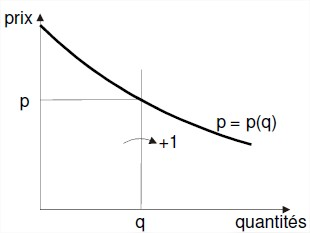
\includegraphics[scale=0.5]{1-6CourbeDem.jpg}
				\caption{}\label{fig:demand_curve}
			\end{figure}

			\begin{empheq}[box=\widefbox]{alignat*=2}
				&u_i(q) \: \textcolor{vert}{\nearrow} \textnormal{ si } q \:
				\textcolor{vert}{\nearrow} \textnormal{, soit } u_i'(q) &&> 0\\
				&u_i'(q) \: \textcolor{red}{\searrow} \textnormal{ si } q \:
				\textcolor{vert}{\nearrow} \textnormal{, soit } u_i''(q) &&< 0
			\end{empheq}
		\end{mydef}
		\bigbreak


		\begin{mydef}[\textcolor{violet2}{\underline{Coût total}}]
			 Montant nécessaire à la production d'un bien ou d'un service.
			 Il est égal à l'intégrale du coût marginal.

			\begin{figure}[H]
				\centering
				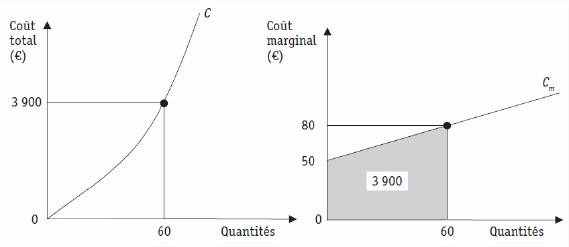
\includegraphics[scale=0.6]{1-6CoutTot.jpg}
				\caption{Coût total et coût marginal.}
				\label{fig:total_cost}
			\end{figure}
		\end{mydef}
		\bigbreak


		\begin{mydef}[\textcolor{violet2}{\underline{Disposition à consommer}}]
			S'il existe un seul prix, l'acheteur est prêt à consommer toutes les unités pour lesquelles \textcolor{miorangerouge}{$u'_i(q) > p$}.
		\end{mydef}
		\bigbreak


		\begin{mydef}[\textcolor{violet2}{\underline{Disposition marginale à payer}} (\textcolor{miorangerouge}{$u'_i(q)$})]
			Elle désigne la façon dont un consommateur donné estime
			l'ordre de grandeur de prix qu'il est prêt à payer
			pour acquérir et consommer un bien ou un service donné.
			\begin{itemize}[label={\color{violet} \textbullet}]
				\item Elle $\textcolor{red}{\searrow}$ si
				$\textcolor{miorangerouge}{q} \: \textcolor{vert}{\nearrow}$.
				\item \textbf{Satiété} : $\textcolor{miorangerouge}{u''_i(q) < 0} \implies \left\{
				\begin{array}{ll}
					u'_i(q) &\textcolor{red}{\textnormal{décroissante }} \textnormal{avec } \textcolor{miorangerouge}{q}, \\
					p &\textcolor{red}{\textnormal{décroissant}}.
				\end{array}
				\right.$
			\end{itemize}

			\begin{figure}[H]
				\centering
				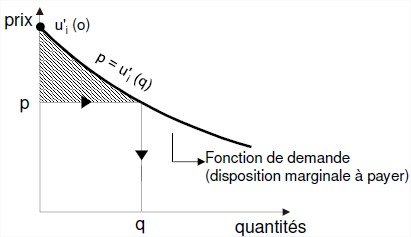
\includegraphics[scale=0.5]{1-6DispositionMargP.jpg}
				\caption{}\label{fig:wtp} % willingness to pay
			\end{figure}

		\end{mydef}
		\bigbreak


		\begin{mydef}[\textcolor{violet2}{\underline{Surplus}} (\textcolor{miorangerouge}{$s_i$})]
			Le surplus est l'éxcédent de ce que le consommateur va retirer
			par rapport à ce qu'il paye.
			\begin{itemize}[label={\color{violet} \textbullet}]
				\item \textcolor{miorangerouge}{$s_i = u_i(q) -p \cdot q$}.
				\item $s_i = u_i(q) -p \cdot q = \displaystyle\int_{0}^{q} u'_i(q) \dif q - p \cdot q = \textcolor{miorangerouge}{\displaystyle\int_{0}^{q} p(q) \dif q - p \cdot q}$.
			\end{itemize}
			\begin{mydef}[\textbf{Surplus du consommateur} (\textcolor{miorangerouge}{$\surpluscons $})]
				La \textcolor{blue}{perte} que le consommateur subirait si on lui \textcolor{blue}{enlevait la possibilité d'acheter toutes les quantités au même prix} $p$.
				\begin{itemize}[label={\color{violet} \textbullet}]
					\item $\surpluscons  = \displaystyle\int_{0}^{q_0} p(q) \dif q - p_0 \cdot q_0$.
				\end{itemize}

				\begin{figure}[H]
                  \begin{minipage}[t]{.5\linewidth}
                    \centering
                    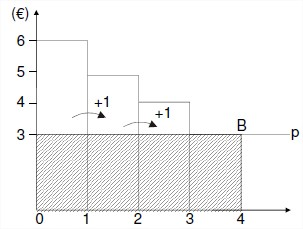
\includegraphics[scale=0.5]{1-6Surplus.jpg}
                    \label{fig:surplusa}
                  \end{minipage}%
                  \begin{minipage}[t]{.5\linewidth}
                    \centering
                    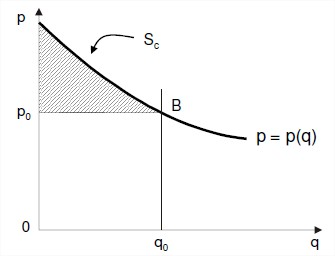
\includegraphics[scale=0.5]{1-6Surplus2.jpg}
                    \label{fig:surplusb}
                  \end{minipage}
                  \caption{Le surplus.}\label{fig:surplus}
                \end{figure}
			\end{mydef}
		\end{mydef}
		\bigbreak


		\begin{mydef}[\textcolor{violet2}{\underline{Utilité marginale}}]
			L'utilité marginale d'un bien ou d'un service est
			l'utilité qu'un agent économique tirera
			de la consommation d'une quantité supplémentaire
			de ce bien ou de ce service.
			\begin{itemize}[label={\color{violet} \textbullet}]
				\item La dernière unité consommée aura une valeur
				exactement égale au prix.
				Après, ce n'est plus intéressant.
				\item Détermine la valeur d'un bien.
			\end{itemize}
		\end{mydef}
		\bigbreak


		\begin{mydef}[\textcolor{violet2}{\underline{Utilité retirée de la consommation d'un bien}}]
			Il y a deux écoles:
			\begin{itemize}[label={\color{violet} \textbullet}]
				\item \textbf{école classique} : valeur d'un bien (\textcolor{miorangerouge}{$q$} unités) = $\sum$ des coûts;
				\item \textbf{école néo-classique} : valeur d'un bien (\textcolor{miorangerouge}{$q$} unités)
				= \textcolor{miorangerouge}{$u_i(q)$} (\textcolor{vert}{croissante})
				= ce que l'acheteur est prêt à payer en fonction de l'utilité qu'il peut en retirer.
				\begin{myrem}
					L'acheteur essaye d'avoir une utilité
					la plus grande possible par rapport à ce qu'il paye
					$\implies$ \textcolor{blue}{maximisation} du surplus \textcolor{miorangerouge}{$\max\limits_q \: u_i(q) -p \cdot q$}.
				\end{myrem}
			\end{itemize}
		\end{mydef}
		\bigbreak






		%%%%%%%%%%%%%%%%%%%%%%%%%%%%%%%%%%%%%%%%%%%%%%%%%%%%%%%%%%%%%%%%%%%%%%%%%%%%%%%%%

	\subsection{Élasticité de la demande par rapport au prix} % 1.7


		\begin{mydef}[\textcolor{violet2}{\underline{Élasticité d'un bien}} (\textcolor{miorangerouge}{$\elasticity (q,p)$})]\leavevmode
			\begin{itemize}[label={\color{violet} \textbullet}]
				\item \textcolor{miorangerouge}{$\elasticity (q,p) = \lim\limits_{\Delta p \to 0} \displaystyle\frac{\Delta q/q}{\Delta p/p} = \displaystyle\frac{\dif q/q}{\dif p/p}$}.
				\item Rapport de la variation relative de la demande d'un bien
				à la variation relative du prix de ce bien.
				\item Ce qui mesure la sensibilité qu'a la demande du bien
				par rapport à son prix.
				\item Manière dont la demande d'un bien évolue par rapport à son prix.
				\item Pas d'unités $\longrightarrow \left[ \displaystyle\frac{\%}{\%} \right]$.
				\item Négative normalement car $\displaystyle\frac{-}{+} $.

				\begin{myrem}
					Sauf pour les biens de Giffen
					$\rightarrow$ au plus le prix du pain augmentait,
					au plus on en consommait (paradoxe de Giffen).
					Si on effectue plus de ponctions sur les revenus des gens,
					ils n'ont plus assez d'argent donc ne peuvent acheter que du pain.
				\end{myrem}
			\end{itemize}
		\end{mydef}
		\bigbreak

		\begin{mydef}[\textcolor{violet2}{\underline{Bien élastique}}]
			Bien dont l'élasticité est très élevée.
			Quand on bouge les prix,
			la demande change énormément.
			La courbe de demande est peu pentue.
			Un bien inélastique peut devenir très élastique
			si c'est un bien qui devient industriel.
		 	\begin{myexem}
		 		Électricité.
		 	\end{myexem}

			\begin{figure}[H]
				\centering
				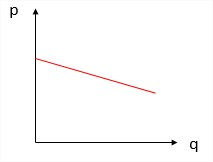
\includegraphics[scale=0.5]{1-7elast.jpg}
				\caption{Courbe de demande d'un bien élastique.}
				\label{fig:elastic_demand}
			\end{figure}
		\end{mydef}
		\bigbreak


		\begin{mydef}[\textcolor{violet2}{\underline{Bien inélastique}}]
			Bien dont l'élasticité est très basse.
			Quand on bouge les prix,
			la demande ne change presque pas.
			La courbe de demande est très pentue.
			\begin{myexem}
				Carburants (pétrole),
				produits agricoles (blé, café, cacao,\dots).
			\end{myexem}

			\begin{figure}[H]
				\centering
				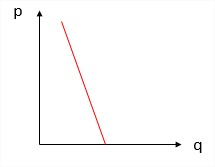
\includegraphics[scale=0.5]{1-7inelast.jpg}
				\caption{Courbe de demande d'un bien inélastique.}
				\label{fig:inelastic_demand}
			\end{figure}
		\end{mydef}
		\bigbreak


		\begin{mydef}[\textcolor{violet2}{\underline{Bien inférieur}}]
			Si le prix \textcolor{vert}{$\nearrow$} alors la demande \textcolor{vert}{$\nearrow$} aussi (bien de Giffen).
			\begin{myexem}
				Pain.
			\end{myexem}
		\end{mydef}
		\bigbreak


		\begin{mydef}[\textcolor{violet2}{\underline{Bien supérieur}}]
			Si le prix \textcolor{red}{$\searrow$}
			alors la demande \textcolor{red}{$\searrow$} aussi (effet Veblen).
			\begin{myexem}
				Montre Patek Philippe.
			\end{myexem}
		\end{mydef}
		\bigbreak


		%%%%%%%%%%%%%%%%%%%%%%%%%%%%%%%%%%%%%%%%%%%%%%%%%%%%%%%%%%%%%%%%%%%%%%%%%%%%%%%%%

	\subsection{Fonctions de coût à court terme (CT)} % 1.8


		\begin{mydef}[\textcolor{violet2}{\underline{Coût fixe}} (\textcolor{miorangerouge}{$C(0)$, $\cfixe $})]
			Coût en $t = 0$,
			indépendant de la production de l'entreprise.
			Il s'additionne au coût variable.
		\end{mydef}
		\bigbreak

		\begin{mydef}[\textcolor{violet2}{\underline{Coût variable}} (\textcolor{miorangerouge}{$\cvar (q)$})]
			Le coût variable est le coût qui varie
			plus ou moins proportionnellement à l’activité de l’entreprise.
		\end{mydef}
		\bigbreak


		\begin{mydef}[\textcolor{violet2}{\underline{Coût marginal}} (\textcolor{miorangerouge}{$\cmarg (q)$})]\leavevmode
			\begin{itemize}[label={\color{violet} \textbullet}]
				\item Coût lié à la prise de décision.
				\item \textcolor{miorangerouge}{$\cmarg (q) \coloneqq \displaystyle\frac{\dif C(q)}{\dif q}$} $= \cmoy  + q \cdot \displaystyle\frac{\dif \cmoy }{\dif q} = \cmoyvar  + q \cdot \displaystyle\frac{\dif \cmoyvar }{\dif q}$.
				\item Pente de la \textcolor{blue}{tangente} $\left(\displaystyle\frac{\dif C(q_A)}{\dif q} = \tan \beta \right)$.
				\begin{myrem}
					Si on diminue la pente le plus possible tout en touchant la courbe,
					la sécante devient égale à la tangente
					et le coût moyen devient égal au coût marginal
					(\textcolor{miorangerouge}{$\cmoy  = \cmarg $}).
				\end{myrem}
			\end{itemize}

			\begin{figure}[H]
				\begin{minipage}[t]{.5\linewidth}
					\centering
					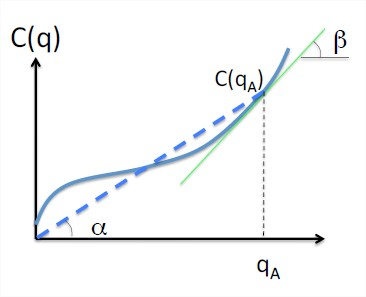
\includegraphics[scale=0.5]{tansec.jpg}
					\label{fig:tanseca}
				\end{minipage}%
				\begin{minipage}[t]{.5\linewidth}
					\centering
					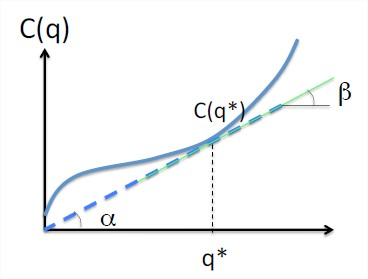
\includegraphics[scale=0.5]{tansec2.jpg}
					\label{fig:tansecb}
				\end{minipage}
				\caption{}\label{fig:tansec}
			\end{figure}
		\end{mydef}
		\bigbreak


		\begin{mydef}[\textcolor{violet2}{\underline{Coût moyen}} (\textcolor{miorangerouge}{$\cmoy (q)$})]\leavevmode
			\begin{itemize}[label={\color{violet} \textbullet}]
				\item $\cmoy (q) = \displaystyle\frac{\textnormal{coût total}}{\textnormal{quantité}}$.
				\item \textcolor{miorangerouge}{$\cmoy (q) \coloneqq \displaystyle\frac{C(q)}{q}$} $= \displaystyle\frac{\cfixe +\cvar (q)}{q} = \displaystyle\frac{\cfixe }{q}+\cmoyvar  = \cmoyfixe + \cmoyvar $.
				\item Pente de la \textcolor{blue}{sécante} $\left(\displaystyle\frac{C(q_A)}{q} = \tan \alpha \right)$. \begin{myrem}
					Si on diminue la pente le plus possible
					tout en touchant la courbe,
					la sécante devient égale à la tangente
					et le coût moyen devient égal au coût marginal
					(\textcolor{miorangerouge}{$\cmoy  = \cmarg $}).
				\end{myrem}
				\item $\fdif{\cmoy}{q} < 0 \implies \cmarg  < \cmoy \longrightarrow$
				Productivité moyenne \textcolor{vert}{croissante}, coût moyen \textcolor{red}{décroissant}.
				\item $\fdif{\cmoy}{q} > 0 \implies \cmarg  > \cmoy  \longrightarrow$ Productivité moyenne \textcolor{red}{décroissante}, coût moyen \textcolor{vert}{croissant}.
				\item $\fdif{\cmoy}{q} = 0 \implies \cmarg  = \cmoy  \longrightarrow$ Au point où la productivité moyenne passe par un maximum, le coût moyen est minimum.
			\end{itemize}
		\end{mydef}
		\bigbreak

		\begin{figure}[H]
			\centering
			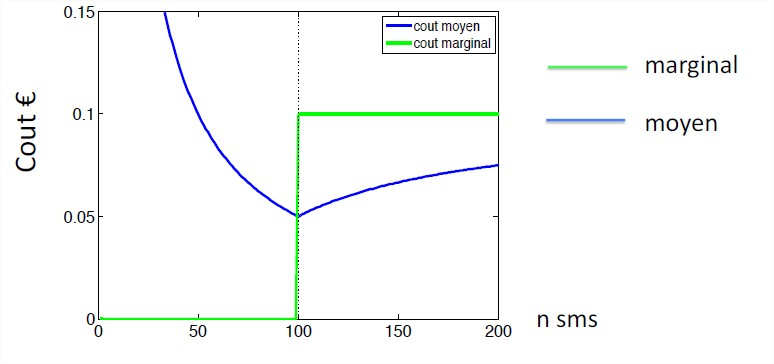
\includegraphics[scale=0.4]{coutmargmoy1.jpg}
			\caption{Coûts moyen et marginal pour un abonnement téléphonique.}
			\label{fig:marg_avg_cost}
		\end{figure}
		\bigbreak

		\begin{mydef}[\textcolor{violet2}{\underline{Coût moyen fixe}} (\textcolor{miorangerouge}{$\cmoyfixe$})] \textcolor{miorangerouge}{$\cmoyfixe = \displaystyle\frac{\cfixe }{q}$}
		\end{mydef}
		\bigbreak

		\begin{mydef}[\textcolor{violet2}{\underline{Coût moyen variable}} (\textcolor{miorangerouge}{$\cmoyvar $})]\leavevmode
			\begin{itemize}[label={\color{violet} \textbullet}]
				\item \textcolor{miorangerouge}{$\cmoyvar  = \displaystyle\frac{\cvar (q)}{q}$}.
				\item $\fdif{\cmoyvar}{q} < 0 \implies \cmarg  < \cmoyvar $.
				\item $\fdif{\cmoyvar}{q} > 0 \implies \cmarg  > \cmoyvar $.
				\item $\cmarg $ passe par le minimum de $\cmoy $ et de $\cmoyvar $:
				\begin{itemize}[label={\color{Orchid} \textbullet}]
					\item $\min \cmoy  \implies \fdif{\cmoy}{q} = 0 \implies \cmarg  = \cmoy $.
					\item $\min \cmoyvar  \implies \fdif{\cmoyvar}{q} = 0 \implies \cmarg  = \cmoyvar $.
				\end{itemize}
			\end{itemize}
		\end{mydef}
		\bigbreak


		\begin{mydef}[\textcolor{violet2}{\underline{Coût total}} (\textcolor{miorangerouge}{$C(q)$})]\leavevmode
			\begin{itemize}[label={\color{violet} \textbullet}]
				\item Coût pour produire une quantité $q$ (toujours positive).
				\item \textcolor{miorangerouge}{$C(q) = C(0) + \displaystyle\int_{0}^{q} \cmarg  (\tilde{q}) \dif \tilde{q} = \cfixe  + \cvar (q)$}
				\qquad Coût total = coût fixe + coût variable.
			\end{itemize}
		\end{mydef}
		\bigbreak


		\begin{mydef}[\textcolor{violet2}{\underline{Point d'efficacité maximale}} (\textcolor{miorangerouge}{$\qopt $})]
			Intersection entre le coût moyen et le coût marginal
			(\textcolor{miorangerouge}{$\cmoy  = \cmarg$}).

			\begin{figure}[H]
				\centering
				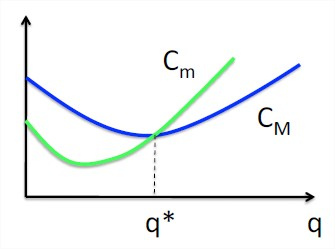
\includegraphics[scale=0.4]{PtEffMax.jpg}
				\caption{Le point d'efficacité maximale.}\label{fig:point_eff_max}
			\end{figure}

		\end{mydef}
		\bigbreak


		\begin{mydef}[\textcolor{violet2}{\underline{Rendements d'échelle (dé)croissants}}]
			Dans le cas des rendements d'échelle croissants, si on \textcolor{vert}{augmente} l'argent mis dans la production (on \textcolor{red}{$\searrow$} le coût marginal), c'est plus efficace (+ d'unités produites).
			\begin{myexem}
				Si c'est plus rentable, on a intérêt à avoir une grosse usine.
			\end{myexem}
			Le cas de figure opposé est celui des rendements d'échelle décroissants.


			\begin{itemize}[label={\color{violet} \textbullet}]
				\item \textbf{Croissants}

				\begin{figure}[H]
					\centering
					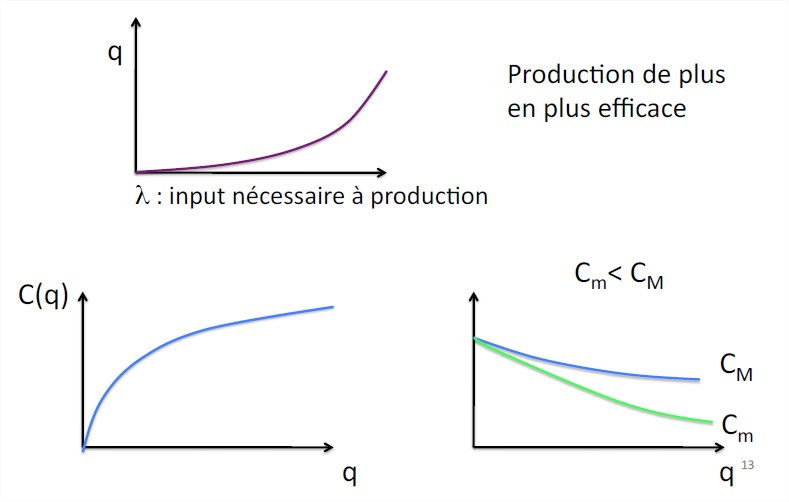
\includegraphics[scale=0.4]{RECroissants.jpg}
					\caption{}\label{fig:rec}
				\end{figure}

				\item \textbf{Décroissants}

					\begin{figure}[H]
					\centering
					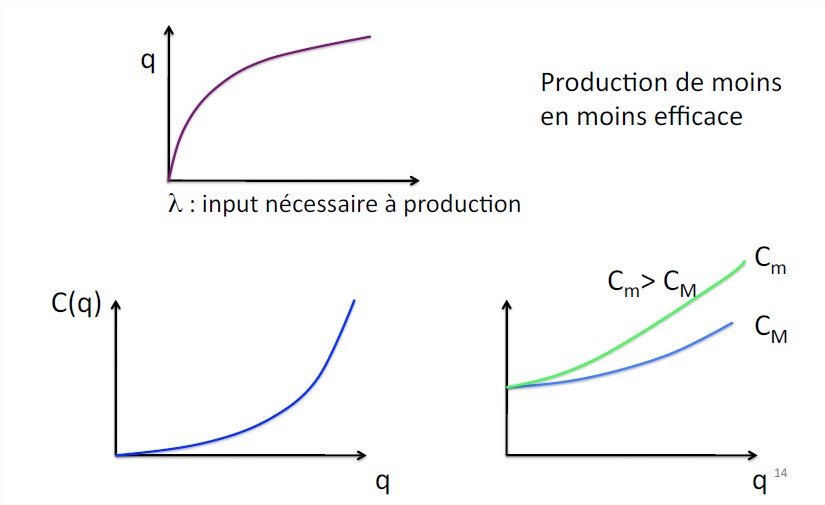
\includegraphics[scale=0.4]{REDecroissants.jpg}
					\caption{}\label{fig:red}
				\end{figure}
			\end{itemize}
		\end{mydef}
		\bigbreak


		\begin{mydef}[\textcolor{violet2}{\underline{Sunk cost}}]
			Coût qui a déjà été payé définitivement.
			Ils n'est ni remboursable,
			ni récupérable par un autre moyen.
			\begin{myexem}
				Coût fixe de 10, coût variable de $q$. $C(q) = 10 + q \implies \textnormal{SC} = 10$.
			\end{myexem}
		\end{mydef}
		\bigbreak


		%%%%%%%%%%%%%%%%%%%%%%%%%%%%%%%%%%%%%%%%%%%%%%%%%%%%%%%%%%%%%%%%%%%%%%%%%%%%%%%%%

	\subsection{Analyse de court terme et de long terme} % 1.9


		\begin{mydef}[\textcolor{violet2}{\underline{$\lambda^*$}} ($\lambda$ stable)]
			Taille optimale (de l'usine) en fonction de la quantité à produire.
		\end{mydef}
		\bigbreak


		\begin{mydef}[\textcolor{violet2}{\underline{Court terme}}]
			Marché où seules
			les quantités de \textcolor{blue}{facteurs variables} de production
			peuvent faire l'objet de décisions des entreprises.
			\begin{itemize}[label={\color{violet} \textbullet}]
				\item Seules certaines variables peuvent être ajustées.
				\item Grande importance des décisions déjà prises.
				\item Capacité de production fixe.
				\item Technologies invariantes.
				\item (Nombre de firmes sur le marché fixé.)
			\end{itemize}
		\end{mydef}
		\bigbreak



		\begin{mydef}[\textcolor{violet2}{\underline{Coût marginal de court terme}} (étant donné une installation adaptée à $\qopt$) (\textcolor{miorangerouge}{$C_{\textnormal{m,CT}}(q \suchthat \qopt)$})]
			Coût de production d'une unité supplémentaire
			\textcolor{blue}{en gardant un équipement adapté à $\qopt$}.
		\end{mydef}
		\bigbreak

		\begin{mydef}[\textcolor{violet2}{\underline{Coût marginal de long terme}} (\textcolor{miorangerouge}{$C_{\textnormal{m,LT}}$})]\leavevmode
			\begin{itemize}[label={\color{violet} \textbullet}]
				\item \textcolor{miorangerouge}{$C_{\textnormal{m,LT}}(q) = \fpart{C_{\textnormal{LT}}(q)}{q}$}.
				\item Coût de production d'une unité supplémentaire \textcolor{blue}{en adaptant l'équipement à $q+1$}.
				\item Pente de la tangente en un point à $C(q,\lambda)$.
			\end{itemize}
		\end{mydef}
		\bigbreak

		\begin{mydef}[\textcolor{violet2}{\underline{Coût moyen de court terme}} (courbe de) (\textcolor{miorangerouge}{$C_{\textnormal{M,CT}}$})]
			Donne le coût unitaire pour
			différents niveaux de production
			pour \textcolor{blue}{une période de temps donnée}.
		\end{mydef}
		\bigbreak

		\begin{mydef}[\textcolor{violet2}{\underline{Coût moyen de long terme}} (\textcolor{miorangerouge}{$C_{\textnormal{M,LT}}$})]\leavevmode
			\begin{itemize}[label={\color{violet} \textbullet}]
				\item \textcolor{miorangerouge}{$C_{\textnormal{M,LT}}(q) = \displaystyle\frac{C_{\textnormal{LT}}(q)}{q}$}.
				\item Pente du vecteur de l'origine.
			\end{itemize}
		\end{mydef}
		\bigbreak


		\begin{mydef}[\textcolor{violet2}{\underline{Coût total}} (\textcolor{miorangerouge}{$C(q,\lambda)$})]
			Coût pour produire une quantité $q$.
			\begin{myrem}
				Chaque usine (= unité de production)
				se caractérise par une \textcolor{blue}{technologie}
				et une \textcolor{blue}{taille},
				réductibles à un paramètre \textcolor{miorangerouge}{$\lambda$}.
			\end{myrem}


			\begin{figure}[H]
				\centering
				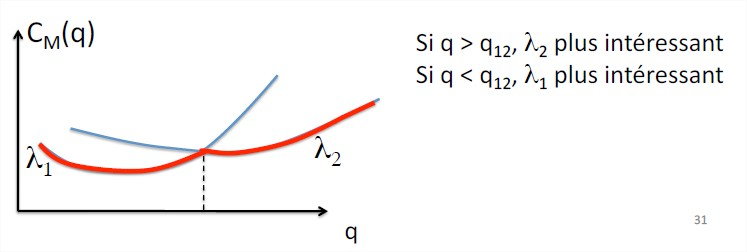
\includegraphics[scale=0.4]{lambdaentreprise.jpg}
				\caption{}\label{fig:lambda_firm}
			\end{figure}
		\end{mydef}
		\bigbreak


		\begin{mydef}[\textcolor{violet2}{\underline{Coût total de court terme}} (courbe des dépenses totales de CT)]\leavevmode \textcolor{miorangerouge}{$D(q,\lambda) = A(\lambda) + B(q,\lambda)$}
			\begin{itemize}[label={\color{violet} \textbullet}]
				\item \textcolor{miorangerouge}{$A(\lambda)$} = charges totales de capital supportées par unité de temps (et frais fixes).
				\item \textcolor{miorangerouge}{$B(q,\lambda)$} = charges d'exploitation liées à la fois à la production courante et à la taille des installations.
				\item \underline{Condition d'adaptation des usines à un niveau de production quelconque}:
				\[
					\textcolor{miorangerouge}{\fpart{D(q,\lambda)}{\lambda} = 0}
					\qquad \textnormal{ou} \qquad
					\textcolor{miorangerouge}{\fdif{A}{\lambda} + \fpart{
					B(q,\lambda)}{\lambda} = 0}.
				\]
			\end{itemize}
		\end{mydef}
		\bigbreak


		\begin{mydef}[\textcolor{violet2}{\underline{Coût total de court terme}} (étant donné une installation adaptée à $\qopt$) (\textcolor{miorangerouge}{$C_{CT}(q \suchthat \qopt)$})]
			\label{def:CT_total_cost}
			Coût de production d'une quantité $q$ \textcolor{blue}{avec un équipement adapté à $\qopt $}.
		\end{mydef}
		\bigbreak



		\begin{mydef}[\textcolor{violet2}{\underline{Coût total de long terme}} (\textcolor{miorangerouge}{$C_{\textnormal{LT}}(q)$})]\leavevmode
			\begin{itemize}[label={\color{violet} \textbullet}]
				\item \textcolor{miorangerouge}{$C_{\textnormal{LT}}(q) = D(\lambda^*(q),q)$}.
				\item $C_{\textnormal{LT}} =$ coût si l'équipement est adapté $\longrightarrow C_{\textnormal{m,LT}}(q) = C_{\textnormal{m,CT}}(q)$.
				\item Minimiser les dépenses totales (optimisation).

				\begin{myexem}
					300 smartphones en 2 ans
					$\longrightarrow$ on choisit la meilleure taille d'usine.
				\end{myexem}
				\item Égal à l'enveloppe des coûts à court terme.
				\item Si on peut prendre toutes les décisions que l'on veut, coût total optimal.
			\end{itemize}

			\[
				\boxed{C_{\textnormal{LT}}(q) \le C_{\textnormal{CT}}(q \suchthat \qopt) \textnormal{ avec l'égalité uniquement si } q = \qopt.}
			\]

			C'est logique,
			car par définition tous les deux sont égaux
			au coût de produire avec un équipement de production adapté à $\qopt$.
			L'inégalité provient donc du fait que
			la production avec un équipement inadapté
			n'est jamais plus efficace
			qu'avec un équipement adapté.


			\begin{figure}[H]
				\centering
				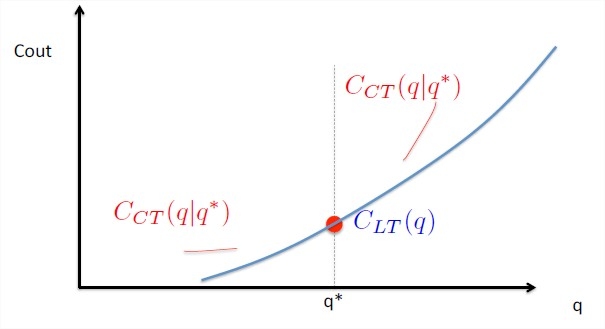
\includegraphics[scale=0.4]{CoutTotLT1.jpg}
				\caption{}\label{fig:LTtotal_cost}
			\end{figure}
		\end{mydef}
		\bigbreak


		\begin{mydef}[\textcolor{violet2}{\underline{Enveloppe}} (\textcolor{miorangerouge}{$E$})]
			Si \textcolor{miorangerouge}{$\lambda$} varie ``continûment'',
			on peut tracer l'enveloppe des dépenses totales
			\textcolor{miorangerouge}{$C(q,\lambda)$}.
			(Dépenses à long terme de l'entreprise.)
		\end{mydef}
		\bigbreak

		\begin{mydef}[\textcolor{violet2}{\underline{Équipements adaptés}} (ensemble des)]
			Famille de courbes à un paramètre dans le plan $(D,q)$,
			qui admettent une enveloppe \textcolor{miorangerouge}{$E$},
			dont l'équation s'obtient
			en éliminant \textcolor{miorangerouge}{$\lambda$}
			entre les deux équations (``lieu'') (voir coût total de court terme, Définition~\ref{def:CT_total_cost}).
		\end{mydef}
		\bigbreak


		\begin{mydef}[\textcolor{violet2}{\underline{Long terme}}]
			Les \textcolor{blue}{technologies et capacités s'ajustent},
			mais pas le nombre d'entreprises (marchés protégés).
			\begin{itemize}[label={\color{violet} \textbullet}]
				\item Tout peut changer.
				\item Peu d'influence des décisions déjà prises.
				\item Les capacités installées s'adaptent à la production demandée.
				\item Les technologies évoluent.
				\item (Des firmes entrent et sortent du marché.)
			\end{itemize}
		\end{mydef}
		\bigbreak


		\begin{mydef}[\textcolor{violet2}{\underline{Niveau d'équipement}} (d'une entreprise)]\leavevmode
			\begin{itemize}[label={\color{violet} \textbullet}]
				\item \textbf{Exactement adaptée} au volume $q_0$ visé:
				$q = \qopt  \implies C_{\textnormal{m,CT}}(q \suchthat \qopt)
				= C_{\textnormal{m,LT}}(q)$.
				\item \textbf{Suréquipée}:
				$q < \qopt  \implies C_{\textnormal{m,CT}}(q \suchthat \qopt)
				\le C_{\textnormal{m,LT}}(q)$.
				($\Delta q$ à CT est peu onéreux.)
				\item \textbf{Sous-équipée}:
				$q > \qopt  \implies C_{\textnormal{m,CT}}(q \suchthat \qopt)
				\ge C_{\textnormal{m,LT}}(q)$.
				(Il est plus avantageux d'augmenter la capacité.)
			\end{itemize}

			\begin{figure}[H]
				\centering
				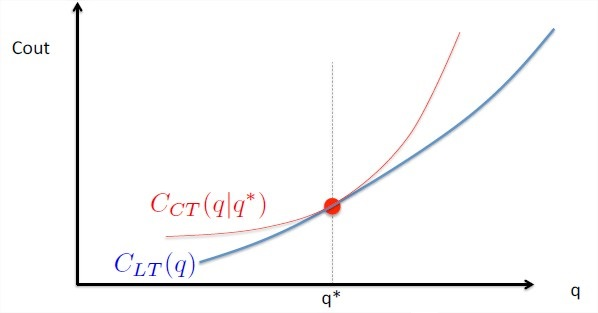
\includegraphics[scale=0.45]{NivEq1.jpg}
				\caption{}\label{fig:niveq}
			\end{figure}
		\end{mydef}
		\bigbreak


		\begin{mydef}[\textcolor{violet2}{\underline{Zone optimale}}]
			Zone où les coûts moyens sont les + faibles.
		\end{mydef}



		%%%%%%%%%%%%%%%%%%%%%%%%%%%%%%%%%%%%%%%%%%%%%%%%%%%%%%%%%%%%%%%%%%%%%%%%%%%%%%%%%

	\subsection{Prise en compte explicite du temps} % 1.10


		\begin{mydef}[\textcolor{violet2}{\underline{$\sigma$}}]
			Variation de ce que l'on pense vendre.
		\end{mydef}
		\bigbreak


		\begin{mydef}[\textcolor{violet2}{\underline{Effet d'accélération}}]
			L'entreprise est d'autant plus soumise aux répercussions
			qu'elle se situe plus en \textcolor{blue}{amont}
			dans le système de production.
			Au plus loin (\textcolor{vert}{$\nearrow$} d'étapes intermédiaires) on est du client,
			au plus les répercussions seront importantes.

			\begin{figure}[H]
				\centering
				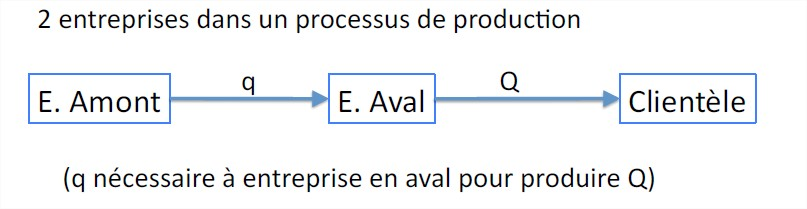
\includegraphics[scale=0.35]{effetacc1.jpg}
				\caption{}\label{fig:acc_effect}
			\end{figure}


			\begin{itemize}[label={\color{violet} \textbullet}]
				\item \textbf{Facteur de production non stockable}: \textcolor{miorangerouge}{$q_t = K \cdot Q_t$}

				La conjoncture affecte également amont et aval.
				\item \textbf{Facteur de production stockable} (matières premières, semi-finis, équipement):
				\begin{itemize}[label={\color{Orchid} \textbullet}]
					\item \textcolor{miorangerouge}{$q_t = K \cdot Q_t$}.
					\item \textbf{Stock} (\textcolor{miorangerouge}{$S$}): $\textcolor{miorangerouge}{S_t = \sigma \cdot Q_{t+1}} \implies
					\textcolor{miorangerouge}{\Delta S = \sigma \cdot \Delta Q}$.
				\end{itemize}
				\item \textbf{Demande totale de} $\bm{q}$ (pendant la période $\Delta t = \interval{t}{t+1}$) :
				\begin{itemize}[label={\color{Orchid} \textbullet}]
					\item consommation effective à la période $t$;
					\item augmentation de stock provenant de l'effet d'anticipation : \textcolor{miorangerouge}{$q_t = K \cdot Q_t + \sigma \cdot \Delta Q_t$}.

					Si $\Delta t \to 0$, on a la quantité consommée entre $t$ et $t+\dif tt$ : \textcolor{miorangerouge}{$q_t \cdot \dif t = K \cdot Q_t \cdot \dif t + \sigma \cdot \fdif{Q_t}{t} \cdot \dif t$}.
				\end{itemize}
				\item \textbf{Solutions} :
				\begin{itemize}[label={\color{Orchid} \textbullet}]
					\item intégration verticale;
					\item croissance externe et diversification.
				\end{itemize}
			\end{itemize}
		\end{mydef}
		\bigbreak


		\begin{mydef}[\textcolor{violet2}{\underline{Intégration verticale}}]\leavevmode
			\begin{itemize}[label={\color{violet} \textbullet}]
				\item \textbf{But} : atténuer les à-coups.
				\item Tout faire soi-même pour maîtriser toute la chaîne.
				\begin{myrem}
					On ne sait pas forcément tout faire.
				\end{myrem}
			\end{itemize}
		\end{mydef}
		\bigbreak



		\begin{mydef}[\textcolor{violet2}{\underline{Learning curve}}]\leavevmode
			\begin{itemize}[label={\color{violet} \textbullet}]
				\item \textbf{Constat}:
				le coût moyen tend à décroître au \textcolor{blue}{cours du temps}.
				Au plus on produit,
				au plus la courbe de coût se déplace vers le bas.
				On devient meilleur.
				\item Coût par unité produite en fonction du volume \textcolor{blue}{cumulé} de production
				depuis le lancement du process.
				\begin{myexem}
					Diminution d'un \% stable chaque fois que la valeur cumulée de production double.
				\end{myexem}
			\end{itemize}
		\end{mydef}
		\bigbreak



		\begin{mydef}[\textcolor{violet2}{\underline{Production d'amont}}]
			Fonction linéaire de la \textcolor{blue}{production d'aval}
			et de la \textcolor{blue}{dérivée de cette production d'aval}
			(dont le ``poids'' est d'autant plus important
			que le ``stockage'' est plus intense).
		\end{mydef}
		\bigbreak


		%%%%%%%%%%%%%%%%%%%%%%%%%%%%%%%%%%%%%%%%%%%%%%%%%%%%%%%%%%%%%%%%%%%%%%%%%%%%%%%%%

	\subsection{Production avec plusieurs facteurs} % 1.11


		\begin{mydef}[\textcolor{violet2}{\underline{$\lambda$}}]
			À l'optimum,
			si l'on multiplie les facteurs de production de $\delta x = (\delta x_1, \delta x_2,\dots)$
			entraînant un coût additionnel $\delta C = \displaystyle\sum_{i} p_i \delta x_i $,
			la production varie de $\delta Q = \lambda^{-1} \delta C$.

			La production augmente donc de $\left(\lambda^{-1}\right)^*$
			(investissement additionnel),
			quelle que soit la répartition de cet investissement.

			\[
				\displaystyle \frac{\delta Q}{\delta C} = \lambda^{-1}.
			\]

		\end{mydef}
		\bigbreak



		\subsubsection{Choix optimal des facteurs}

			\begin{itemize}[label={\color{violet} \textbullet}]
				\item $\min\limits_{x_1,x_2,\dots}  \displaystyle\sum_{i} p_i x_i $ sous contrainte \textcolor{miorangerouge}{$g(x_1,x_2,\dots) = Q$}.
				\item \textbf{Lagrangien} : \textcolor{miorangerouge}{$\: \displaystyle\sum_{i} p_i x_i + \lambda (Q - g(x_1,x_2,\dots))$}.
				\item \textbf{Conditions d'optimalité} : \textcolor{miorangerouge}{$p_i = \lambda \fpart{g(\bm{x})}{x_i}$}, donc : \textcolor{miorangerouge}{$\lambda^{-1} = \displaystyle\frac{1}{p_i}  \fpart{g(\bm{x})}{x_i}$} \qquad \qquad $\forall i = 1,2,\dots$
				\begin{itemize}[label={\color{Orchid} \textbullet}]
					\item $\fpart{g(\bm{x})}{x_i}=$ taux d'augmentation de la \textcolor{blue}{production}
					par unité du \textcolor{blue}{facteur $x_i$},
					les autres facteurs restant constants.
					\item $\displaystyle\frac{1}{p_i}  \fpart{g(\bm{x})}{x_i} =  \fpart{g(\bm{x})}{(p_i x_i)} =$
					taux d'augmentation
					de la \textcolor{blue}{production par \euro{} additionnel} inverti dans $x_i$,
					les autres facteurs restant constants.
					\item À l'optimum, le taux est le même pour tous les facteurs.
					\item \textbf{Non-unicité} : conditions nécessaires mais pas suffisantes pour que $\bm{x}$ soit optimal.
					Il est possible que plusieurs répartitions les satisfassent.
					Dans ce cas, il faut sélectionner
					une de celles menant au coût le plus faible.
				\end{itemize}
				\item L'ensemble des solutions définit le chemin des facteurs adaptés, paramétrés par $\textcolor{miorangerouge}{Q}$.
			\end{itemize}

		\subsubsection{Coûts}

			\begin{mydef}[\textcolor{violet2}{\underline{Coût}}] \textcolor{miorangerouge}{$C = \displaystyle\sum_{i} p_i x_i $}.
				\begin{itemize}[label={\color{violet} \textbullet}]
					\item \textbf{Facteurs de production} : $x_1, x_2, \dots$
					\item \textbf{Prix de ces facteurs} : $p_1, p_2, \dots$
				\end{itemize}
			\end{mydef}
			\bigbreak

			\begin{mydef}[\textcolor{violet2}{\underline{Coût marginal}} (\textcolor{miorangerouge}{$\lambda$})]\leavevmode
			\begin{itemize}[label={\color{violet} \textbullet}]
				\item \textcolor{miorangerouge}{$\lambda = \displaystyle \frac{\delta C}{\delta Q}$}.
				\item Indépendant de la façon dont sont répartis les facteurs de production additionnels.

				\begin{myexem}
					Investissement dans les personnes ou les matériaux.
				\end{myexem}
			\end{itemize}


			\setlength{\fboxsep}{7pt}
			\fbox{\parbox{13.25cm}{
					Au départ d'une situation optimale,
					une (petite) variation \textcolor{miorangerouge}{$\delta q$}
					de la quantité produite reviendra toujours
					à un prix \textcolor{miorangerouge}{$\lambda \delta q$},
					\textcolor{blue}{quelle que soit la façon dont cette variation est obtenue},
					c'est-à-dire quelle que soit la (petite) variation
					\textcolor{miorangerouge}{$\delta x = (\delta x_1, \delta x_2, \dots)$}
					qui réalisera cette variation de production.
			}}

			\end{mydef}
			\bigbreak


			\begin{mydef}[\textcolor{violet2}{\underline{Coût marginal CT-LT}}]\leavevmode
				\begin{itemize}[label={\color{violet} \textbullet}]
					\item \textcolor{miorangerouge}{$x_1, \dots,  x_c$} sont modifiables à court terme.
					\item \textcolor{miorangerouge}{$x_{c+1}, \dots,  x_n$} sont modifiables seulement sur le long terme.
					\item Une (petite) augmentation \textcolor{miorangerouge}{$\delta q$} de la quantité produite aura le même coût si elle est réalisée en modifiant uniquement les facteurs de \textcolor{blue}{court terme} ou en modifiant \textcolor{blue}{tous les facteurs}.
					\item À l'optimum: $\boxed{\textnormal{Coût marginal LT = Coût marginal CT.}}$
				\end{itemize}
			\end{mydef}
			\bigbreak


			\begin{mydef}[\textcolor{violet2}{\underline{Quantité totale produite}}]
				\textcolor{miorangerouge}{$Q = g(x_1,x_2,\dots)$}.
			\end{mydef}
			\bigbreak


			\begin{mydef}[\textcolor{violet2}{\underline{Raisonnement à la marge}}]
				Regarder si cela fonctionne mieux pour un facteur que pour un autre.
				Nous ne sommes pas alors à l'optimal.
				\begin{myexem}
					Mettre \euro{} $\! 10$ dans les personnes et pas les matériaux.
					Attention à la saturation (pas de nombre de personnes négatif).
				\end{myexem}

				\[
					\textcolor{miorangerouge}{\displaystyle\frac{1}{p_i}  \fpart{g(\bm{x})}{x_i} = \displaystyle\frac{1}{p_j}  \fpart{g(\bm{x})}{x_j}} \qquad \forall i,j
				\]


				Supposons par l'absurde, qu'à l'optimum, $\displaystyle\frac{1}{p_i}  \fpart{g(\bm{x})}{x_i} > \displaystyle\frac{1}{p_j}  \fpart{g(\bm{x})}{x_j}$.

				Alors \textcolor{vert}{$\nearrow$} $x_i$ de $\displaystyle\frac{\delta}{p_i}$ et \textcolor{red}{$\searrow$} $x_j$ de $\displaystyle\frac{\delta}{p_j}$ provoque:
				\begin{itemize}[label={\color{violet} \textbullet}]
					\item \textbf{variation de coût}  $= p_i \displaystyle\frac{\delta}{p_i} + p_j \displaystyle\frac{\delta}{p_j} = 0$;
					\item \textbf{variation de production} $\approx$ $ \fpart{g(\bm{x})}{x_i} \displaystyle\frac{\delta}{p_i} -  \fpart{g(\bm{x})}{x_j} \displaystyle\frac{\delta}{p_j} > 0$.

					$\implies$ On produit plus pour le même coût $\longrightarrow$ situation initiale pas optimale.
				\end{itemize}
			\end{mydef}
			\bigbreak



			\begin{mydef}[\textcolor{violet2}{\underline{Saturation}}]\leavevmode
				\begin{itemize}[label={\color{violet} \textbullet}]
					\item Les quantités doivent souvent être positives et peuvent saturer : \textcolor{miorangerouge}{$0 \le x_i \le \widebar{x_i}$}
					\item \textbf{À l'optimum} :
						\begin{align*}
						\displaystyle\frac{1}{p_i} \fpart{g(\bm{x})}{x_i} = \lambda^{-1} & \textnormal{ si } 0 < x_i < \widebar{x_i}, \\
						\displaystyle\frac{1}{p_i}  \fpart{g(\bm{x})}{x_i} \le \lambda^{-1} & \textnormal{ si } x_i=0, \\
						\displaystyle\frac{1}{p_i}  \fpart{g(\bm{x})}{x_i} \ge \lambda^{-1} & \textnormal{ si } x_i = \widebar{x_i}. \\
					\end{align*}
				\end{itemize}
			\end{mydef}
			\bigbreak


		%%%%%%%%%%%%%%%%%%%%%%%%%%%%%%%%%%%%%%%%%%%%%%%%%%%%%%%%%%%%%%%%%%%%%%%%%%%%%%%%%

	\subsection{Comportement de l'entreprise en concurrence parfaite} % 1.12


		\begin{mydef}[\textcolor{violet2}{\underline{Fonction d'offre}}]\leavevmode
			\begin{itemize}[label={\color{violet} \textbullet}]
				\item Le prix est donné quel que soit la quantité demandée
				(dans les hypothèses de concurrence parfaite)
				à l'intersection entre la courbe d'offre globale
				et celle de demande globale.
				\item Si $p$ est trop bas, $q=0$: l'entreprise ne produit pas.

				$C(q) = \cfixe  + \cvar  (q)$.

				Si $q=0$ : $\pcompt(q) = -\cfixe $.
				\item L'entreprise ne produira que si :

				$\pcompt(q) = p \cdot q - \cfixe  - \cvar  (q) \ge - \cfixe  \qquad \textnormal{ ou } \qquad p \ge \displaystyle\frac{\cvar (q)}{q} \qquad \textnormal{ ou } \qquad p \ge C_{\textnormal{VM}} (q)$.
			\end{itemize}
		\bigbreak


			\begin{figure}[H]
				\centering
				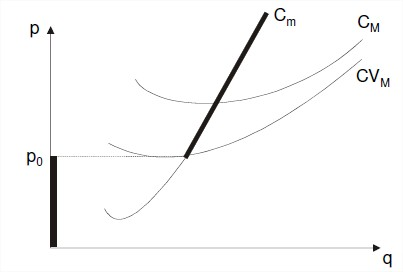
\includegraphics[scale=0.5]{1-11FonctionOffre.jpg}
				\caption{}\label{fig:supply_curve}
			\end{figure}
		\end{mydef}
		\bigbreak


		\begin{mydef}[\textcolor{violet2}{\underline{Maximisation du profit}}]
			La maximisation du profit est le problème d'optimisation suivant:
			\textcolor{miorangerouge}{$\max\limits_q \pi(q) = \max\limits_q p \cdot q - C(q)$}.

			Soit : $\pcompt'(q) = p - \fdif{C}{q} = 0 \implies \textcolor{miorangerouge}{p = \cmarg (q)}$.

			$\pcompt ''(q) = - \ffdif{C}{q} \le 0 \implies \textcolor{miorangerouge}{\cmarg '(q) > 0}$ \qquad \qquad
			À l'\textcolor{blue}{optimum},
			le $\cmarg$ est \textcolor{vert}{croissant}.
		\end{mydef}
		\bigbreak


		\begin{mydef}[\textcolor{violet2}{\underline{PIB}}]
			Richesse créée par l'économie du pays.
		\end{mydef}
		\bigbreak

		\begin{mydef}[\textcolor{violet2}{\underline{Profit}} (\textcolor{miorangerouge}{$\pcompt (q)$})]
			$\textcolor{miorangerouge}{\pcompt (q) = p \cdot q - C(q) }
			= \textnormal{prix de vente} \cdot  q - \textnormal{coût de production}
			= \textnormal{recette} - \textnormal{coût de production}$.

			\begin{figure}[H]
				\centering
				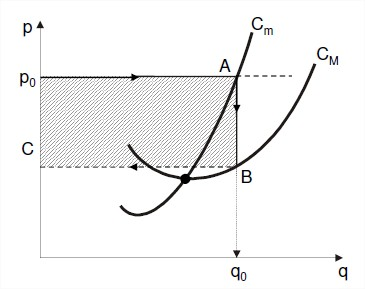
\includegraphics[scale=0.5]{1-11Profit.jpg}
				\caption{}\label{fig:profit}
			\end{figure}
		\end{mydef}
		\bigbreak



		%%%%%%%%%%%%%%%%%%%%%%%%%%%%%%%%%%%%%%%%%%%%%%%%%%%%%%%%%%%%%%%%%%%%%%%%%%%%%%%%%

	\subsection{L'équilibre en concurrence parfaite} % 1.13


		\begin{mydef}[\textcolor{violet2}{\underline{Amortissement}}]
			Chaque année,
			déduit du compte des résultats que dans $x$ années,
			on fera faillite.
		\end{mydef}
		\bigbreak


		\begin{mydef}[\textcolor{violet2}{\underline{Charge financière}}]
			Emprunt à rembourser.
		\end{mydef}
		\bigbreak


		\begin{mydef}[\textcolor{violet2}{\underline{Demande d'une entreprise (CT)}}]\leavevmode
			\begin{itemize}[label={\color{violet} \textbullet}]
				\item Si $p_2 > p_{\textnormal{M}} \quad \longrightarrow \quad$
				\textcolor{blue}{Perte} de tous les \textcolor{blue}{clients} et retour à
				\textcolor{miorangerouge}{$p_{\textnormal{M}}$}.
				\item Si $p_1 < p_{\textnormal{M}} \quad \longrightarrow \quad$
				Toute la clientèle vient chez lui et sa demande est celle du \textcolor{blue}{marché} ($DD'$) :

				Il y a \textcolor{blue}{excès} de \textcolor{blue}{demande} ($AB$),
				ce qui pousse le prix vers
				$p_{\textnormal{M}}$.
			\end{itemize}


			\begin{figure}[H]
				\centering
				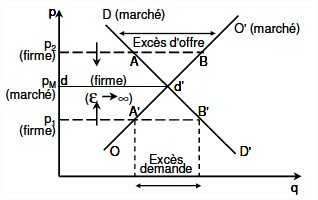
\includegraphics[scale=0.65]{1-12Demande.jpg}
				\caption{}\label{fig:CTdemand}
			\end{figure}
		\end{mydef}
		\bigbreak


		\begin{mydef}[\textcolor{violet2}{\underline{Équilibre (CT)}}]\leavevmode
			\begin{itemize}[label={\color{violet} \textbullet}]
				\item Offre totale = demande totale.
				\item Ce qui correspond à un prix \textcolor{miorangerouge}{$p_{\textnormal{M}}$} tel que \textcolor{miorangerouge}{$O(p_{\textnormal{M}}) =
				D(p_{\textnormal{M}})$}.
				\item Équilibre réalisé pour $q_i$ correspondant à $p_{\textnormal{M}} = C_{\textnormal{m},i}$.
			\end{itemize}

			\begin{figure}[H]
				\centering
				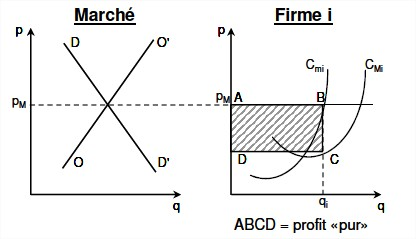
\includegraphics[scale=0.6]{1-12Equilibre1.jpg}
				\caption{}\label{fig:equilibrium}
			\end{figure}
		\end{mydef}
		\bigbreak



		\begin{mydef}[\textcolor{violet2}{\underline{Équilibre (LT)}}]\leavevmode
			\begin{itemize}[label={\color{violet} \textbullet}]
				\item $\pcompt > 0$ $\implies$
				nouveau concurrents attirés dans la branche $\implies$
				offre \textcolor{vert}{$\nearrow$}
				($O_1 \to O_2$ et $p_1 \to p_2$).
				\item En situation initiale, $\pcompt_A$ et $\pcompt_B > 0$,
				car $p_1 > C_{\textnormal{M},A}$ et $p_1 > C_{\textnormal{M},B}$.
				\item Après l'entrée de nouveaux concurrents:
				$p_2 \sim C_{\textnormal{M},A} \implies \pcompt_A \sim 0$
				et $p_2 < C_{\textnormal{M},B} \implies \pcompt_B < 0$.
				\item Offre \textcolor{vert}{$\nearrow$} $\implies$ B sort du marché $\implies$ hausse des prix $\implies$ nouveaux entrants $\implies$ \dots
				\item Ces entrées/sorties finissent quand $\pcompt_i \to 0$ c'est-à-dire quand $p_{\textnormal{M}} = \min C_{\textnormal{M,LT}}$.
				\item À l'équilibre, le profit économique (\textcolor{miorangerouge}{$\ppur$}) de LT est égal à 0.
				L'entreprise n'a pas intérêt à sortir
				et les autres n'ont pas intérêt à rentrer dans son marché.
			\end{itemize}

			\begin{figure}[H]
				\centering
				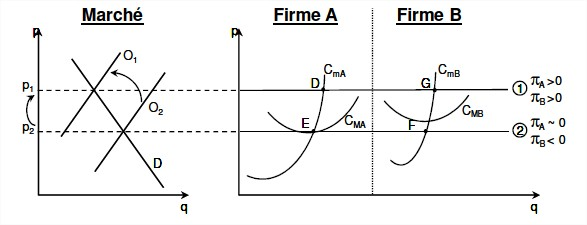
\includegraphics[scale=0.6]{1-12Equilibre2.jpg}
				\caption{}\label{fig:LTequil}
			\end{figure}

		\end{mydef}
		\bigbreak


		\begin{mydef}[\textcolor{violet2}{\underline{Offre d'une entreprise (CT)}}]
			Quantité qu'elle est disposée à produire/vendre pour un prix donné:
			$q = q(p)$.
		\end{mydef}
		\bigbreak

		\begin{mydef}[\textcolor{violet2}{\underline{Profit comptable}} (\textcolor{miorangerouge}{$\pi_{\textnormal{C}}$})]
			Il se réfère aux produits et coûts explicites.
			\begin{myexem}
				Listing, répertoire,\dots
			\end{myexem}
		\end{mydef}
		\bigbreak


		\begin{mydef}[\textcolor{violet2}{\underline{Profit économique}} (\textcolor{miorangerouge}{$\ppur$})]
			$\textcolor{miorangerouge}{\pi_{\textnormal{C}}} + \textnormal{coûts d'opportunité}$.
			\begin{myexem}
				Salaire non perçu,\dots
			\end{myexem}

			\begin{table}[H]
				\centering
				\renewcommand{\arraystretch}{1}
				\begin{tabular}{l l}
					\hline
					$\ppur > 0$ & $i$ gagne plus que dans la meilleure opportunité.\\
					&\\
					\multirow{2}{*}{$\ppur = 0$} & Ne veut pas dire que $i$ fait des pertes.\\
					                    & $i$ gagne autant que ce qu'elle pourrait gagner dans d'autres secteurs.\\
					&\\
					$\ppur < 0$ & Logiquement, la firme $i$ sort du marché.\\
					\hline
				\end{tabular}
			\end{table}
		\end{mydef}
		\bigbreak


		\begin{mydef}[\textcolor{violet2}{\underline{Provisions}}]
			Prévoir ce que les personnes ne payent pas.
		\end{mydef}
		\bigbreak


		%%%%%%%%%%%%%%%%%%%%%%%%%%%%%%%%%%%%%%%%%%%%%%%%%%%%%%%%%%%%%%%%%%%%%%%%%%%%%%%%%

	\subsection{Équilibre et optimum collectif} % 1.14



		\begin{mydef}[\textcolor{violet2}{\underline{Optimum collectif}}]\leavevmode
			\begin{itemize}[label={\color{violet} \textbullet}]
				\item Un \textcolor{blue}{optimum} est atteint
				lorsque le bien est vendu à son coût marginal \textcolor{miorangerouge}{$p = \cmarg $}.
				\item Mesure le gain net global apporté par \textcolor{blue}{ce marché} à l'ensemble consommateurs + producteurs.
			\end{itemize}

			\begin{figure}[H]
				\centering
				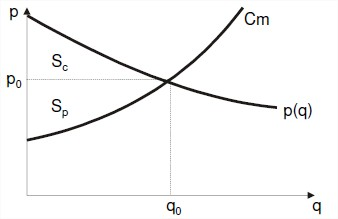
\includegraphics[scale=0.55]{1-13OptimumCol.jpg}
				\caption{}\label{fig:coll_opti}
			\end{figure}


			\begin{itemize}[label={\color{violet} \textbullet}]
				\item $\max\limits_{q_0} S \implies \fpart{S}{q_0} = \fpart{}{q_0}\left(  \displaystyle\int_{0}^{q_0} p(q) \dif q - \displaystyle\int_{0}^{q_0} \cmarg (q) \dif q \right) = 0$.
				\bigbreak
				\item $\max\limits_{q_0} S \implies \textcolor{miorangerouge}{p(q_0) = \cmarg (q_0)}$.
				\item La vente \textcolor{blue}{spontanée} au $\cmarg$ (pour maximiser $\pcompt$).
				\item Production \textcolor{blue}{spontanée} de \textcolor{miorangerouge}{$q_0$} tel que $p = \cmarg (q_0)$.
				\item Maximisent spontanément le surplus collectif.
				\item Maximisation du surplus individuel $\to$ optimum collectif (main invisible/du diable).
			\end{itemize}
		\end{mydef}
		\bigbreak



		\begin{mydef}[\textcolor{violet2}{\underline{Profit des producteurs}} (\textcolor{miorangerouge}{$\pi(q)$})]
			C'est le \textcolor{blue}{supplément de gain} apporté aux producteurs \textcolor{blue}{par le marché en question},
			par différence avec les autres utilisations possibles de leurs moyens financiers.
		\end{mydef}
		\bigbreak


		\begin{mydef}[\textcolor{violet2}{\underline{Situation d'équilibre}}]
			Situation dont aucun des acteurs n'a intérêt à sortir.
		\end{mydef}
		\bigbreak



		\begin{mydef}[\textcolor{violet2}{\underline{Surplus collectif}} (\textcolor{miorangerouge}{$S$})]\leavevmode
			\begin{itemize}[label={\color{violet} \textbullet}]
				\item \textcolor{miorangerouge}{$S = \surpluscons  + \surplusprod $}.
				\item Mesure le gain net global apporté par \textcolor{blue}{ce marché}
				à l'ensemble consommateurs + producteurs.
				\item Marché d'autant plus efficace que le surplus collectif est grand $\implies \max\limits_{q_0} S = \textnormal{optimum collectif}$.
			\end{itemize}


			\begin{figure}[H]
				\centering
				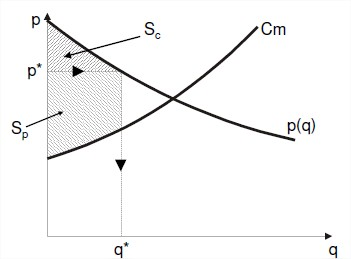
\includegraphics[scale=0.55]{1-13SurplusCol.jpg}
				\caption{}\label{fig:coll_surplus}
			\end{figure}
		\end{mydef}
		\bigbreak



		\begin{mydef}[\textcolor{violet2}{\underline{Surplus des consommateurs}} (\textcolor{miorangerouge}{$\surpluscons $})]\leavevmode
			\begin{itemize}[label={\color{violet} \textbullet}]
				\item \textcolor{miorangerouge}{$\surpluscons  = \displaystyle\int_{0}^{\qopt } p(q) \dif q - \popt  \cdot \qopt$}.
				\item Excédent d'utilité par rapport au prix que le consommateur paye.
			\end{itemize}
		\end{mydef}
		\bigbreak


		\begin{mydef}[\textcolor{violet2}{\underline{Surplus des producteurs}} (\textcolor{miorangerouge}{$\surplusprod$})]\leavevmode
			\begin{itemize}[label={\color{violet} \textbullet}]
				\item\textcolor{miorangerouge}{$\surplusprod  = \pi(\qopt) =$} $\popt \cdot  \qopt  - C(\qopt ) =$ \textcolor{miorangerouge}{$\displaystyle\int_{0}^{\qopt } \cmarg (q) \dif q$}.
				\item Excédent de ce que le producteur reçoit $-$ la somme de ses coûts.
				Si $\popt $ est supérieur au coût marginal,
				le profit est \textcolor{vert}{positif}.
			\end{itemize}
		\end{mydef}


		%%%%%%%%%%%%%%%%%%%%%%%%%%%%%%%%%%%%%%%%%%%%%%%%%%%%%%%%%%%%%%%%%%%%%%%%%%%%%%%%%

	\subsection{États d'équilibre général et états optimaux d'une économie} % 1.15


		\begin{mydef}[\textcolor{violet2}{\underline{Économie utilitariste}}]
			Satisfaction de l'un ou de l'autre inintéressante
			mais la somme qui est la plus grande possible est intéressante.
		\end{mydef}
		\bigbreak


		\begin{mydef}[\textcolor{violet2}{\underline{Équilibre général}} (d'un point de vue explicatif)]\leavevmode
			\begin{itemize}[label={\color{violet} \textbullet}]
				\item Sous les hypothèses de concurrence parfaite.
				\item S'il y a :
				\begin{itemize}[label={\color{Orchid} \textbullet}]
					\item \textcolor{miorangerouge}{$k$} produits ou services (\textcolor{miorangerouge}{$k$} marchés);
					\item \textcolor{miorangerouge}{$m$} consommateurs (utilités, revenus);
					\item \textcolor{miorangerouge}{$n$} producteurs (fonctions de production, coûts facteurs),
				\end{itemize}
				\item alors, il existe un système de prix \textcolor{miorangerouge}{$p_j \quad \forall j = 1,\dots,k$}
				qui équilibre $O$ et $D$ sur chaque marché
				et qui maximise utilités et profits.
				\item Les seuls éléments d'information
				nécessaires à un agent pour prendre ses décisions
				sont les \textcolor{blue}{prix} \textcolor{miorangerouge}{$p_j$} ("décentralisation" des décisions).
				\item Cet état réalise un \textcolor{blue}{optimum collectif}, par maximalisation des surplus $S = \surpluscons  + \surplusprod$.
			\end{itemize}
		\end{mydef}
		\bigbreak


		\begin{mydef}[\textcolor{violet2}{\underline{Équilibre général}} (d'un point de vue normatif)]
			L'optimum de V. Pareto, les ``théorèmes du Welfare''.
			Comment ça devrait se passer\dots{}
			Voilà ce qu'il faut faire.
			\paragraph{Attention} Il y a des limites à l'économie.

			\begin{mytheo}[Théorème de Walras]
				Une économie peut être décentralisée.
				Besoin juste de connaître le prix.
				\begin{myrem}
					Certains utilisent ça
					pour dire que l'état n'est pas nécessaire à l'économie
					car on arrive à un surplus maximal spontanément.
				\end{myrem}

				\begin{figure}[H]
					\centering
					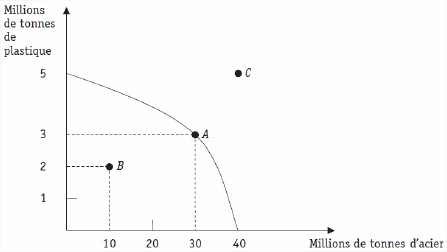
\includegraphics[scale=0.6]{1-14EquilibreWalras.jpg}
					\caption{}\label{fig:walras}
				\end{figure}

				\begin{itemize}[label={\color{violet} \textbullet}]
				\item $B$ : Ressources sous-utilisées.
				\item $A$ : Économie utilise toutes les ressources.
				\item $C$ : Impossible.
				\end{itemize}
			\end{mytheo}

			\begin{itemize}[label={\color{violet} \textbullet}]
				\item \textbf{Pareto}: un état (physiquement) possible est dit
				\textcolor{blue}{pareto-optimal}
				si on ne peut \textcolor{vert}{$\nearrow$} la satisfaction d'un individu
				sans diminuer celle d'un autre.

				\begin{figure}[H]
					\centering
					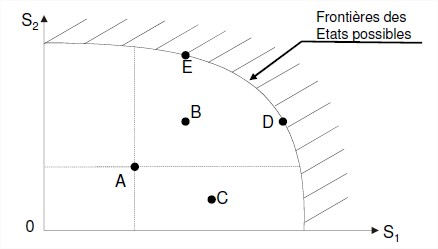
\includegraphics[scale=0.55]{1-14EquilibreNorm.jpg}
					\caption{}\label{fig:equil_norm}
				\end{figure}

				\begin{itemize}[label={\color{Orchid} \textbullet}]
					\item Un point qui n'est pas une frontière ne peut être un optimum de Pareto, car au moins un point de la frontière lui est préférable.
					\item \textbf{Équilibre et optimum de Pareto} :
					\begin{itemize}[label={\color{Thistle} \textbullet}]
						\item tout équilibre de marché réalise un optimum de Pareto;
						\item sous certaines conditions, un optimum de Pareto peut être réalisé par un équilibre de marché.
					\end{itemize}

					\item $A$, $B$ et $C$: pas optimum de Pareto. On peut \textcolor{vert}{$\nearrow$} la satisfaction des deux agents.
					\item $E$ et $D$: optimum de Pareto.
				\end{itemize}

				\item \textbf{Jugement d'équité/d'efficacité}: une économie peut être pareto-efficace même lorsqu'il y a des très riches et des très pauvres tant que les pauvres ne peuvent pas être rendus meilleurs sans rendre les riches moins riches.

				\item \textbf{Critère de Rawls}:

				\begin{itemize}[label={\color{Orchid} \textbullet}]
					\item ne demande pas l'égalité (égalitarisme);
					\item raisonnable avant le rationnel;
					\item faire au mieux pour ceux qui ont le moins
					$\implies$ critère du maximin
					(maximiser les minimas en fonction de ce qu'on a).
				\end{itemize}

				\item \underline{\textit{Attention}}: le recours au marché
				a un \textcolor{blue}{coût}.
				C'est dans la \textcolor{blue}{minimisation} de ce coût
				que l'on trouve l'origine et la ``justification'' de l'\textcolor{blue}{entreprise}.
			\end{itemize}
		\end{mydef}


		%%%%%%%%%%%%%%%%%%%%%%%%%%%%%%%%%%%%%%%%%%%%%%%%%%%%%%%%%%%%%%%%%%%%%%%%%%%%%%%%%

	\subsection{Économies et ``déséconomies'' externes} % 1.16


		Pour rappel, le critère $p = \cmarg$ est nécessaire
		pour avoir un pareto-optimum.
		Jusqu'à présent,
		$\cmarg$ a été considéré comme \textcolor{blue}{indépendant de ``l'extérieur''}:
		en l'absence d'économies ou de ``déséconomies'' externes,
		le coût est le même du point vue \textcolor{blue}{privé}
		(chaque producteur)
		et du point de vue \textcolor{blue}{sociétal} (la collectivité).
		\bigbreak


		\begin{mydef}[\textcolor{violet2}{\underline{Avantage collectif d'une transaction}}]
			Avantage qu'en retire la société $-$
			coût collectif que cette transaction engendre.
		\end{mydef}
		\bigbreak


		\begin{mydef}[\textcolor{violet2}{\underline{Avantage social}} (de $q_1 + q_2$)]
			Mesuré par le revenu \textcolor{blue}{total}.

			$p(q_1 + q_2) = \textnormal{montant que les \textcolor{blue}{consommateurs} sont prêts à payer pour l'output}$.
		\end{mydef}
		\bigbreak


		\begin{mydef}[\textcolor{violet2}{\underline{Coût collectif}}]
			$C_1(q_1, q_2) + C_2(q_1, q_2)$.
		\end{mydef}
		\bigbreak


		\begin{mydef}[\textcolor{violet2}{\underline{Coût des producteurs}}]
			$C_1 = C_1(q_1, q_2)$ et $C_2 = C_2(q_1, q_2)$.
		\end{mydef}
		\bigbreak



		\begin{mydef}[\textcolor{violet2}{\underline{Coûts marginaux collectifs}} (\textcolor{miorangerouge}{$\cmarg^{\textnormal{c}}$})]\leavevmode
			\begin{itemize}[label={\color{violet} \textbullet}]
				\item $\fpart{C_1}{q_1} + \fpart{C_2}{q_1}$ et $\fpart{C_1}{q_2} + \fpart{C_2}{q_2}$.
				\item Maximisation de l'avantage collectif $\implies$
				\textcolor{miorangerouge}{$p = \cmarg^{\textnormal{c}}$}.
			\end{itemize}
		\end{mydef}
		\bigbreak


		\begin{mydef}[\textcolor{violet2}{\underline{Coûts marginaux privés}} (\textcolor{miorangerouge}{$\cmarg^{\textnormal{p}}$})]\leavevmode
			\begin{itemize}[label={\color{violet} \textbullet}]
				\item $\fpart{C_1}{q_1}$ et $\fpart{C_2}{q_2}$ .
				\item Maximisation individuelle $\implies$
				\textcolor{miorangerouge}{$p = \cmarg^{\textnormal{p}}$}.
			\end{itemize}
		\end{mydef}
		\bigbreak


		\begin{mydef}[\textcolor{violet2}{\underline{Déséconomie}}]
			Quand un agent est influencé négativement par un autre.
		\end{mydef}
		\bigbreak


		\begin{mydef}[\textcolor{violet2}{\underline{Maximisation de l'avantage collectif}}]
			\textcolor{miorangerouge}{$\max\limits_{q_1, q_2} \pcompt$} avec
			$\pcompt = \pcompt_1 + \pcompt_2 = p (q_1 + q_2) - C_1(q_1, q_2) - C_2(q_1, q_2)$.

			Soit
			\begin{align*}
				\fpart{\pcompt}{q_1} = p - \fpart{C_1}{q_1} - \fpart{C_2}{q_1} = 0,\\
				\fpart{\pcompt}{q_2} = p - \fpart{C_1}{q_2} - \fpart{C_2}{q_2} = 0.\\
			\end{align*}
		\end{mydef}
		\bigbreak


		\begin{mydef}[\textcolor{violet2}{\underline{Maximisation des profits individuels}}]
			$p = \fpart{C_1}{q_1}$ et $p = \fpart{C_2}{q_2}$.
		\end{mydef}
		\bigbreak


		La maximisation du profit de \textcolor{blue}{chaque} opérateur ne conduit donc plus \textcolor{blue}{spontanément} à l'optimum correspondant à $p = \cmarg$!
		\bigbreak

		La maximisation individuelle
		\textcolor{blue}{n'entraîne pas un optimum collectif}
		en cas d'économies ou ``déséconomies'' externes.


		%%%%%%%%%%%%%%%%%%%%%%%%%%%%%%%%%%%%%%%%%%%%%%%%%%%%%%%%%%%%%%%%%%%%%%%%%%%%%%%%%

	\subsection{Productivité des facteurs et rentes} % 1.17


		\begin{figure}[H]
			\centering
			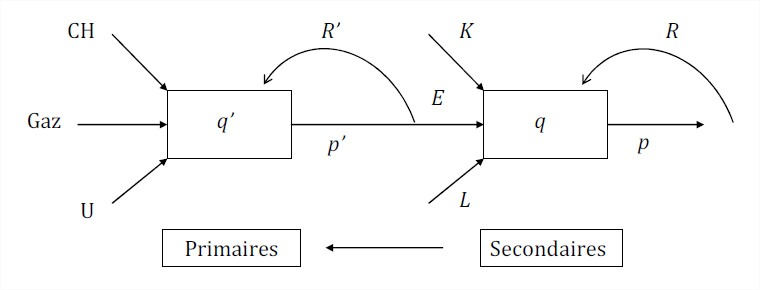
\includegraphics[scale=0.5]{1-16PrimSec.jpg}
			\caption{$K$ = capital, $L$ = travail, $E$ = énergie.}\label{fig:primsec}
		\end{figure}


		\begin{mydef}[\textcolor{violet2}{\underline{Demande de travail}}]
			Les producteurs demandent des employés.
			Au \textcolor{red}{moins} le salaire est haut,
			au \textcolor{vert}{plus} l'offre de demande \textcolor{vert}{$\nearrow$}.
			C'est l'opposé de l'offre de travail.
		\end{mydef}
		\bigbreak



		\begin{mydef}[\textcolor{violet2}{\underline{Maximisation du profit}}]\leavevmode
			\begin{itemize}[label={\color{violet} \textbullet}]
				\item \textbf{1 seul facteur}: $\max \pcompt \implies \fpart{\pcompt}{x} = p \cdot \fpart{q}{x} - p_x = 0$ \quad ou \quad $p \cdot \fpart{q}{x} = p_x$ \quad ou \quad $\fpart{q}{x} \displaystyle\frac{1}{p_x} = \displaystyle\frac{1}{p}$.
				\item On mobilisera donc des quantités de facteur $x$
				jusqu'à ce que sa recette marginale soit égale à son prix,
				ni plus, ni moins.
				\item \textbf{$\bm{n}$ facteurs}: $\fpart{q}{x_1} \displaystyle\frac{1}{p_{x,1}} = \cdots =  \fpart{q}{x} \displaystyle\frac{1}{p_{x,n}} = \displaystyle\frac{1}{p}$.
			\end{itemize}
		\end{mydef}
		\bigbreak



		\begin{mydef}[\textcolor{violet2}{\underline{Offre de travail}}]
			Ce que les employés offrent aux producteurs.
			Au \textcolor{vert}{plus} le salaire est haut,
			au \textcolor{vert}{plus} l'offre de travail $\textcolor{vert}{\nearrow}$.
			C'est donc l'opposé de la demande de travail.
		\end{mydef}
		\bigbreak



		\begin{mydef}[\textcolor{violet2}{\underline{Prix d'un facteur}}]
			En concurrence parfaite,
			le prix d'un facteur est à la fois égal
			à son \textcolor{blue}{coût marginal}
			pour les entreprises qui l'\textcolor{blue}{offrent}
			et à sa \textcolor{blue}{recette marginale}
			pour les entreprises qui le \textcolor{blue}{demandent}.
		\end{mydef}
		\bigbreak




		\begin{mydef}[\textcolor{violet2}{\underline{Productivité marginale}}]\leavevmode
			\begin{itemize}[label={\color{violet} \textbullet}]
				\item $\textcolor{miorangerouge}{\fpart{q}{x}}$.
				\item Supplément de quantité de produit final
				pouvant être fabriqué
				par la mobilisation d'un supplément du facteur $x$.
				\item \textbf{Productivité marginale du facteur travail} : $p \cdot \fpart{q}{L} = w$ \qquad ($w$ est le taux de salaire).
				\item \textbf{Productivité marginale du facteur capital} : $p \cdot \fpart{q}{K} = r$ \qquad ($r$ est le taux d'intérêt).
			\end{itemize}
		\end{mydef}
		\bigbreak



		\begin{mydef}[\textcolor{violet2}{\underline{Profit}} (\textcolor{miorangerouge}{$\pcompt$})]\leavevmode
			\begin{itemize}[label={\color{violet} \textbullet}]
				\item Dans le cas où il n'y a
				qu'\textcolor{blue}{un seul} facteur de production ($p_x$)!
				\item $\textcolor{miorangerouge}{\pcompt} = p \cdot q(x) - C(x) \textcolor{miorangerouge}{\: = p \cdot q(x) - p_x \cdot x}$.

				$p_x$ est le prix unitaire du facteur $x$. $x$ est la quantité mobilisée de ce facteur.
			\end{itemize}
		\end{mydef}
		\bigbreak



		\begin{mydef}[\textcolor{violet2}{\underline{Recette marginale}} (du facteur $x$)]\leavevmode
			\begin{itemize}[label={\color{violet} \textbullet}]
				\item Seulement en \textcolor{blue}{concurrence parfaite} !
				\item $\textcolor{miorangerouge}{\fpart{R}{x} = p \cdot \fpart{q}{x}}$.
			\end{itemize}
		\end{mydef}
		\bigbreak


		\begin{mydef}[\textcolor{violet2}{\underline{Rigidité}} (des facteurs et rentes)]
			Les constats précédents valent
			si les facteurs de production sont ``fluides''
			et \textcolor{blue}{disponibles en quantités limitées}.
		\end{mydef}
		\bigbreak



		%%%%%%%%%%%%%%%%%%%%%%%%%%%%%%%%%%%%%%%%%%%%%%%%%%%%%%%%%%%%%%%%%%%%%%%%%%%%%%%%%

	\subsection{Les imperfections des marchés} % 1.18


		\begin{itemize}[label={\color{violet} \textbullet}]
			\item\textbf{Nombre de vendeurs/acheteurs}:
			\begin{itemize}[label={\color{Orchid} \textbullet}]
				\item certains agents ne prennent pas le prix comme une donnée;
				\item coalitions d'acheteurs ou de vendeurs
				(monopole, duopole, oligopole, coopération d'acheteurs).
			\end{itemize}
			\item L'entrée sur le marché n'est pas toujours \textcolor{blue}{libre}.
			\item \textcolor{blue}{Imperfection de l'information} dont disposent les agents (pas de transparence parfaite).
			\item Pas de théorie unitaire des marchés imparfaits mais des théories partielles correspondant à des situations réelles spécifiques.
		\end{itemize}
		\bigbreak

		%%%%%%%%%%%%%%%%%%%%%%%%%%%%%%%%%%%%%%%%%%%%%%%%%%%%%%%%%%%%%%%%%%%%
		%%%%%%%%%%%%%%%%%%%%%%%%%%%%%%%%%%%%%%%%%%%%%%%%%%%%%%%%%%%%%%%%%%%%
		%%%%%%%%%%%%%%%%%%%%%%%%%% Chapitre 2 %%%%%%%%%%%%%%%%%%%%%%%%%%%%%%
		%%%%%%%%%%%%%%%%%%%%%%%%%%%%%%%%%%%%%%%%%%%%%%%%%%%%%%%%%%%%%%%%%%%%
		%%%%%%%%%%%%%%%%%%%%%%%%%%%%%%%%%%%%%%%%%%%%%%%%%%%%%%%%%%%%%%%%%%%%


\section{Le monopole}
		%%%%%%%%%%%%%%%%%%%%%%%%%%%%%%%%%%%%%%%%%%%%%%%%%%%%%%%%%%%%%%%%%%%%%%%%%%%%%%%
	\subsection{Définitions, caractéristiques et origines} % 2.1



		\subsubsection{Caractéristiques}

			\begin{itemize}[label={\color{violet} \textbullet}]
				\item Étant le seul sur le marché,
				\textcolor{blue}{la demande} qui s'adresse au monopoleur
				est \textcolor{blue}{celle du marché dans son ensemble}.
				\begin{myrem}
					Il peut fixer le prix.
				\end{myrem}
				\item D'où, les décisions de production ($q$) du monopole
				modifient le prix.
				On dit que le monopole possède un ``\textcolor{blue}{pouvoir de marché}''.
				Il n'est donc pas ``price taker''
				(prix à l'intersection entre l'offre et la demande imposé à tous).
				\item Les ventes du monopoleur dépendent uniquement
				de \textcolor{blue}{son} prix
				et du \textcolor{blue}{comportement des consommateurs}.
				\item Il n'est pas nécessaire d'avoir un seul producteur
				mais que le prix soit fixé
				\textcolor{blue}{comme s'il existait un offreur unique}.
				\begin{myexem}
					Le monopole des 7 s\oe{}urs.
				\end{myexem}
			\end{itemize}
			\bigbreak



			\paragraph{Conditions théoriques d'existence d'un monopole pur}\leavevmode

			\begin{itemize}[label={\color{violet} \textbullet}]
				\item \textcolor{blue}{Homogénéité} du produit et \textcolor{blue}{transparence} de l'information.
				\item \textcolor{blue}{Unicité} de l'offre et \textcolor{blue}{atomicité} de la demande.
				\item \textcolor{blue}{Absence} de \textcolor{blue}{libre circulation} des ressources (marché fermé).
				\item \textcolor{blue}{Absence} de \textcolor{blue}{substituts} (montre $\ne$ ordinateur).
			\end{itemize}

		\subsubsection{Définitions}


			\begin{mydef}[\textcolor{violet2}{\underline{Libéraliser}}]
				Lever les monopoles.
			\end{mydef}
			\bigbreak


			\begin{mydef}[\textcolor{violet2}{\underline{Monopole}}]
				Le marché d'un produit est en monopole
				lorsqu'\textcolor{blue}{une seule firme} offre ce produit
				à l'ensemble des consommateurs.
				Il n'y a plus de libre entrée et sortie (plus CP).
			\end{mydef}
			\bigbreak


		\subsubsection{Origines}

			\begin{itemize}[label={\color{violet} \textbullet}]
				\item \textbf{Technologiques} : R\&D, brevets (quelqu'un dispose d'une ressource que personne d'autre n'a), ressources,\dots
				\item \textbf{Institutionnelles} : monopoles légaux (SNCB, Poste, services publics,\dots).
				\item \textbf{Économiques} : étape ultime d'un processus normal de concentrations d'entreprises (Electrabel).
				\item \textbf{Intrinsèques à l'activité} : monopoles naturels (par nature, ne peuvent s'organiser qu'en monopoles).
			\end{itemize}
		\bigbreak



		%%%%%%%%%%%%%%%%%%%%%%%%%%%%%%%%%%%%%%%%%%%%%%%%%%%%%%%%%%%%%%%%%%%%%%%%%%%%%%%%%

	\subsection{Recette et profit du monopole} % 2.2


		\textcolor{violet2}{\underline{Caractéristiques}}

		\begin{itemize}[label={\color{violet} \textbullet}]
			\item La $\rmarg$ s'annule pour un $q$ donné et devient négative $\left(q>\displaystyle\frac{a}{2b}\right)$.
			\item $\rmarg $ a une pente double de celle de la fonction de demande
			(si $p = p(q)$ linéaire).
		\end{itemize}
		\bigbreak


		\begin{figure}[H]
			\centering
			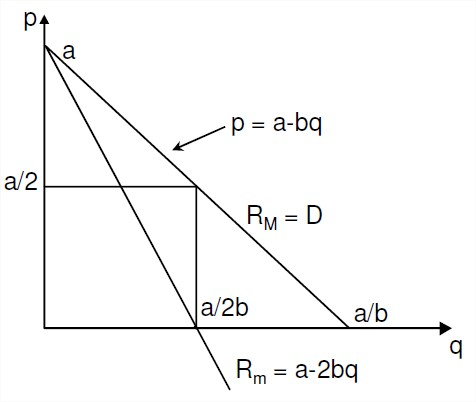
\includegraphics[scale=0.45]{2-2FctDemande.jpg}
			\caption{Fonction de demande (exemple linéaire).}
			\label{fig:demand_curve_ex}
		\end{figure}


		\textcolor{violet2}{\underline{Lien entre fonction de demande et recette marginale}}

		\begin{itemize}[label={\color{violet} \textbullet}]
			\item $\rmarg  = \fdif{}{q}\left(p(q)\cdot q\right) = p(q) + q \cdot  \fdif{p}{q}$
			\item $\fdif{p}{q} < 0 \implies \left\{
			\begin{array}{l}
			\rmarg  < \rmoy  \\
			\rmarg  < p
			\end{array}
			\right.$
			\item Pour rappel, en concurrence parfaite,
			on avait $\rmarg = \rmoy = p$.
			Le monopoleur, lui, pour vendre une unité supplémentaire,
			devra accepter un prix plus bas pour l'ensemble de sa production.
		\end{itemize}
		\bigbreak


		\textcolor{violet2}{\underline{Lien entre $\rmarg $ et élasticité - prix de la demande}}

		\begin{itemize}[label={\color{violet} \textbullet}]
			\item On définit : $\elasticity = \displaystyle\frac{\dif q/q}{\dif p/p}$ ou $\displaystyle\frac{\dif p}{\dif q} = \displaystyle\frac{1}{\elasticity} \cdot \displaystyle\frac{p}{q}$.
			\item $\rmarg  = p(q) + q \cdot  \fdif{p}{q} = p(q) + q \cdot (\displaystyle\frac{1}{\elasticity} \cdot \displaystyle\frac{p}{q}) = p + \displaystyle\frac{p}{\elasticity}$.

			\[
				\boxed{\rmarg = p(q) \cdot \left(1+ \displaystyle\frac{1}{\elasticity}\right)}
			\]

			\item En général, $\elasticity < 0$.
		\end{itemize}
		\bigbreak



		\begin{mydef}[\textcolor{violet2}{\underline{Profit}} (\textcolor{miorangerouge}{$\pcompt$})]\leavevmode
			\begin{itemize}[label={\color{violet} \textbullet}]
				\item \textcolor{miorangerouge}{$\pcompt = R - C$}.
				\item $R$ = recette totale (chiffre d'affaires) : $R=R(q)$.
				\item $C$ = coût total de production : $C = C(q)$.
				\item $\pcompt = \pcompt(q)$.
			\end{itemize}
		\end{mydef}
		\bigbreak


		\begin{mydef}[\textcolor{violet2}{\underline{Recette marginale}} (\textcolor{miorangerouge}{$\rmarg$})]\leavevmode
			\begin{itemize}[label={\color{violet} \textbullet}]
				\item Variation de la recette totale due à la vente d'une unité supplémentaire.
				\item \textcolor{miorangerouge}{$\rmarg  = \fdif{R}{q} = a-2bq$}.
			\end{itemize}
		\end{mydef}
		\bigbreak



		\begin{mydef}[\textcolor{violet2}{\underline{Recette moyenne}} (\textcolor{miorangerouge}{$\rmoy$})]\leavevmode

			\begin{itemize}[label={\color{violet} \textbullet}]
				\item $\textcolor{miorangerouge}{\rmoy} = \displaystyle\frac{R}{q} = \displaystyle\frac{p\cdot q}{q} \textcolor{miorangerouge}{= p}$ = prix de vente unitaire (\textcolor{miorangerouge}{$\rmoy  = p$}).
				\item $\textcolor{miorangerouge}{\rmoy } = \displaystyle\frac{R}{q} = \displaystyle\frac{p\cdot q}{q} = \displaystyle\frac{aq - bq^2}{q} \textcolor{miorangerouge}{= a - bq}$ = fonction de demande (\textcolor{miorangerouge}{$\rmoy  = D$}).
			\end{itemize}
		\end{mydef}
		\bigbreak

		\begin{mydef}[\textcolor{violet2}{\underline{Recette totale}} (\textcolor{miorangerouge}{$R$})]
			\textcolor{miorangerouge}{$R = p\cdot q = aq - bq^2$}.
		\end{mydef}
		\bigbreak


	%%%%%%%%%%%%%%%%%%%%%%%%%%%%%%%%%%%%%%%%%%%%%%%%%%%%%%%%%%%%%%%%%%%%%%%%%%%%%%%%%

	\subsection{Maximisation du profit et détermination du prix} % 2.3


		\subsubsection{Détermination du prix}

			\begin{itemize}[label={\color{violet} \textbullet}]
				\item Fixation \textcolor{blue}{spontanée} d'un prix \textcolor{blue}{supérieur} au $\cmarg$.
				\item Production \textcolor{blue}{spontanée} de la quantité offerte à \textcolor{blue}{$\qmon < q_0$} (perte de Welfare par ``effet Malthusien'').
			\end{itemize}

			\begin{figure}[H]
				\centering
				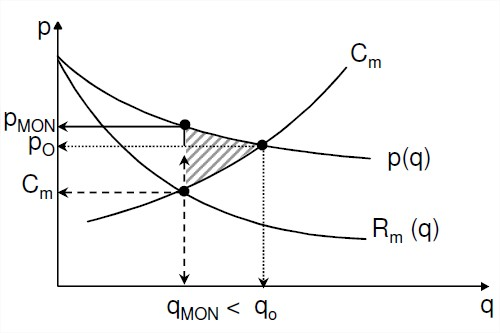
\includegraphics[scale=0.5]{2-3DetPrix1.jpg}
				\caption{}\label{fig:price_det}
			\end{figure}


		\subsubsection{Maximisation du profit}

			\begin{itemize}[label={\color{violet} \textbullet}]
				\item $\pcompt(q) = R(q) - C(q)$.
				\item $\max \pcompt \implies \fdif{\pcompt}{q} = 0 \implies \boxed{\rmarg  = \cmarg}$
				\item $\pcompt(q) = p(q) \cdot q - C(q)$.

				\[
				\fdif{p}{q} = p + q\cdot \fdif{p}{q} - \fdif{C}{q} = 0,
				\]

				\[
				p + q\cdot \fdif{p}{q} = \cmarg,
				\]

				\[
				\fdif{p}{q} < 0 \implies \boxed{p > \cmarg}
				\]
			\end{itemize}
			\bigbreak



	\subsubsection{Représentation graphique des prix et profits}

	\begin{itemize}[label={\color{violet} \textbullet}]
		\item \textbf{À court terme}

		\begin{figure}[H]
			\centering
			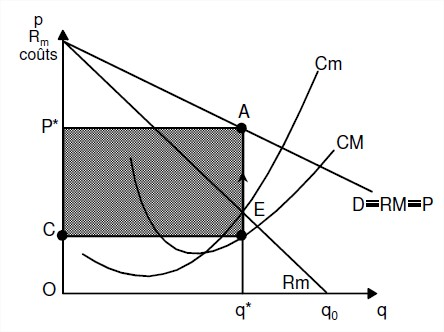
\includegraphics[scale=0.45]{2-3GraphCT.jpg}
			\caption{}\label{fig:graphCT}
		\end{figure}
		\item \textbf{À long terme} : en passant de la taille 0 à la taille 1, le monopole \textcolor{vert}{$\nearrow$} son profit.

		\begin{figure}[H]
			\centering
			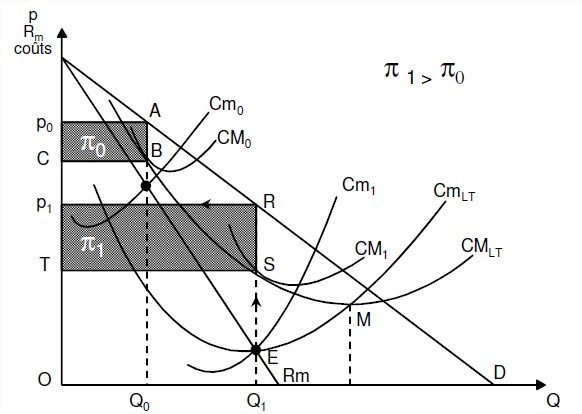
\includegraphics[scale=0.45]{2-3GraphLT.jpg}
			\caption{}\label{fig:graphLT}
		\end{figure}

	\end{itemize}


	%%%%%%%%%%%%%%%%%%%%%%%%%%%%%%%%%%%%%%%%%%%%%%%%%%%%%%%%%%%%%%%%%%%%%%%%%%%%%%%%%

	\subsection{Lien entre prix et coût marginal} % 2.4


		Nous avons $\rmarg  = p(q) \cdot \left(1+ \displaystyle\frac{1}{\elasticity}\right)$ et $\rmarg  = \cmarg$.


		\[
			\boxed{\displaystyle\frac{p-\cmarg}{p} = - \displaystyle\frac{1}{\elasticity} \qquad \text{ ou } \qquad p = \displaystyle\frac{\cmarg }{1+\displaystyle\frac{1}{\elasticity}}} \implies \elasticity < 0 \implies p > \cmarg\,.
		\]

		$\displaystyle\frac{p-\cmarg }{p}$ = ``\textcolor{blue}{mark-up}'' par rapport au $\cmarg $ exprimé en pourcentage du prix.
		De combien peut-on s'éloigner du $\cmarg$?
		Plus la société est grande, moins on peut s'éloigner du $\cmarg$.
		\bigbreak

		Quand un producteur peut vendre son produit
		à un prix \textcolor{blue}{supérieur} à son coût marginal,
		on dit qu'il dispose d'un \textcolor{blue}{pouvoir de marché}
		(\emph{market power}).
		\bigbreak

		Si $\abs{\elasticity} \gg 0 \implies p \sim \cmarg$;
		il y a peu d'avantages à être monopoleur
		si la demande est très élastique.


	%%%%%%%%%%%%%%%%%%%%%%%%%%%%%%%%%%%%%%%%%%%%%%%%%%%%%%%%%%%%%%%%%%%%%%%%%%%%%%%%%

	\subsection{Le monopole à plusieurs établissements} % 2.5


		\textcolor{violet2}{\underline{Principe}}:
		$\boxed{\rmarg  (q_1+q_2) = C_{\textnormal{m},1} = C_{\textnormal{m},2}}$
		\bigbreak

		\begin{mydef}[\textcolor{violet2}{\underline{Rendements croissants et décroissants}}]
			Répartitions optimales de la production entre unités
			(ou entre producteurs).

			\renewcommand{\arraystretch}{1.5} % Espacement dans les cellules = 150% de l'espacement normal pour 1.5
			\begin{table}[H]
				\centering
				\begin{tabular}{p{7.3cm}p{7.3cm}} %\raggedleft, \raggedright et \centering puis plus \\ mais \tabularnewline
					\hline
					\centering{\textcolor{violet2}{\textbf{Croissants}}} & \centering{\textcolor{violet2}{\textbf{Décroissants}}} \tabularnewline
					\centering{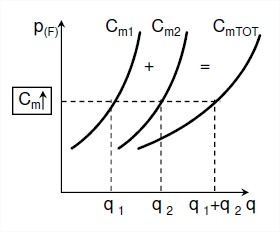
\includegraphics[scale=0.55]{2-5RCroiss.jpg}} & \centering{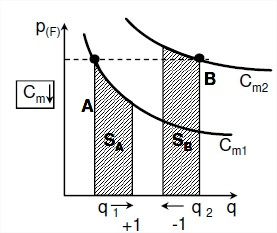
\includegraphics[scale=0.55]{2-5RDecroiss.jpg}} \tabularnewline
					Optimum ($\min D$) $\implies C_{\textnormal{m},1} = C_{\textnormal{m},2}\, .$

					Car si écart existait, il y aurait intérêt à diminuer la production du plus cher jusqu'à l'égalité. & Si $C_{\textnormal{m},1}, C_{\textnormal{m},2} \: \textcolor{red}{\searrow}$ : \begin{itemize}[label={\color{violet} \textbullet}]
						\item économie $S_B >$ supplément $S_A$;
						\item production sur une unité $(q_1 = q_{\mathsc{tot}})$.
					\end{itemize} \\
					& Monopole naturel d'un système de production (voir \sectionref{struct_nat}).\\
					\hline
				\end{tabular}
			\end{table}
		\end{mydef}
		\bigbreak


	%%%%%%%%%%%%%%%%%%%%%%%%%%%%%%%%%%%%%%%%%%%%%%%%%%%%%%%%%%%%%%%%%%%%%%%%%%%%%%%%%

	\subsection{L'``inefficacité sociale'' du monopole} % 2.6



		\begin{itemize}[label={\color{violet} \textbullet}]
			\item Le monopole produit une quantité moindre,
			vendue à un prix plus élevé (effet Malthusien).
			\item Perte de surplus collectif due au monopole.
			\begin{figure}[H]
				\centering
				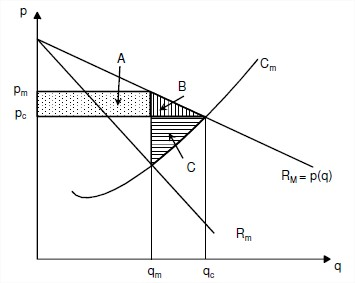
\includegraphics[scale=0.55]{2-6PerteSC.jpg}
				\caption{}\label{fig:perte_sc}
			\end{figure}
			\begin{itemize}[label={\color{Orchid} \textbullet}]
				\item $\bm{A}$ : perte de surplus des \textcolor{blue}{consommateurs},
				parce qu'ils achètent $q_{\textnormal{m}}$ au prix $p_{\textnormal{m}}$
				au lieu de $p_{\textnormal{c}} < p_{\textnormal{m}}$.
				\item $\bm{B}$ : perte de surplus due au fait qu'ils ne peuvent plus acquérir $q_{\textnormal{c}}$,
				mais seulement $q_{\textnormal{m}}$
				(car l'offre est limitée à $q_{\textnormal{m}}$).
				\item $\bm{A+B}$ : perte totale des \textcolor{blue}{consommateurs}
				par rapport à la concurrence parfaite.
				\item $\bm{A}$ : le surplus du \textcolor{blue}{producteur} augmente de $\bm{A}$.
				Mais il aurait vendu en concurrence $q_{\textnormal{c}}$ à $p_{\textnormal{c}}$.
				En monopole, il perd donc $\bm{C}$.
				\item \textbf{Perte de Welfare} ($\bm{B}$ + $\bm{C}$) : perte nette de satisfaction et de profit = \textbf{deadweight loss}.
			\end{itemize}
			\item Le surplus collectif n'est plus maximum
			et donc le monopole n'est pas un marché efficace.
		\end{itemize}
		\bigbreak


		\begin{mydef}[\textcolor{violet2}{\underline{Profit du monopole}} (\textcolor{miorangerouge}{$\pimon$}) (p. 87)]\leavevmode
			\begin{itemize}[label={\color{violet} \textbullet}]
				\item $\pimon  = \left[  \displaystyle\frac{C}{1+1/\elasticity} \right]^{\elasticity+1} \cdot \displaystyle\frac{1}{\elasticity}\,.$
				\item \textbf{Ratio} : $r' = \displaystyle\frac{\pimon }{\sccp} = \left[  \displaystyle\frac{\elasticity}{1+1/\elasticity} \right]^{\elasticity}\,.$
			\end{itemize}
		\end{mydef}
		\bigbreak


		\begin{mydef}[\textcolor{violet2}{\underline{Surplus du consommateur}} (\textcolor{miorangerouge}{$\surpluscons $}) (p. 86)]\leavevmode
			\begin{itemize}[label={\color{violet} \textbullet}]
				\item $\surpluscons = - \displaystyle \frac{(\popt )^{\elasticity+1}}{\elasticity+1}\,.$
				\item \textbf{En concurrence parfaite} : $\sccp  = - \displaystyle \frac{C^{\elasticity+1}}{\elasticity+1}\,.$
				\item \textbf{En monopole} : $\scmon = - \displaystyle \frac{\left[  \displaystyle\frac{C}{1+1/\elasticity} \right]^{\elasticity+1}}{\elasticity+1}\,.$
				\item \textbf{Ratio} : $r = \displaystyle\frac{\scmon}{\sccp } = \left[ \displaystyle\frac{1}{1+1/\elasticity} \right]^{\elasticity+1}\,.$
			\end{itemize}
		\end{mydef}
		\bigbreak


%%%%%%%%%%%%%%%%%%%%%%%%%%%%%%%%%%%%%%%%%%%%%%%%%%%%%%%%%%%%%%%%%%%%%%%%%%%%%%%%%

	\subsection{``Structure naturelle'' d'un marché et d'un monopole naturel} % 2.7
	\label{sec:struct_nat}


		\subsubsection{Structure naturelle}
		
			\begin{itemize}[label={\color{violet} \textbullet}]
			\item Celle qui \textcolor{blue}{minimise le coût global de l'offre} sur ce marché.
			\item Un secteur est un \textcolor{blue}{monopole naturel}
			s'il est plus efficace d'avoir \textcolor{blue}{une seule entreprise}
			qui produit.
			\item \textbf{Cas 1} : $\forall q \colon \cmarg^{\textnormal{LT}} (q) <  \cmoy^{\textnormal{LT}} (q)\,.$
			
				\begin{figure}[H]
					\centering
					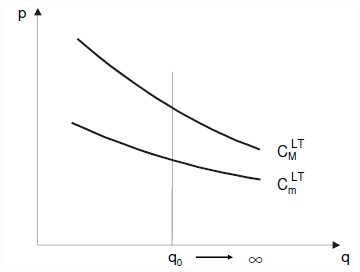
\includegraphics[scale=0.55]{2-7StructNat1.jpg}
					\caption{}\label{fig:struct_nat1}
				\end{figure}
			
				\item \textbf{Cas 2} : Coûts fixes très élevés.
				
				\begin{figure}[H]
					\centering
					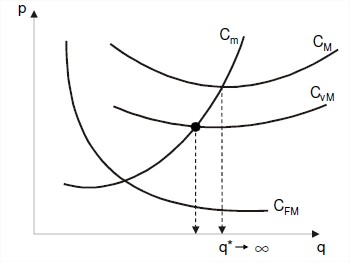
\includegraphics[scale=0.55]{2-7StructNat2.jpg}
					\caption{$\qopt$ tel que $\min\limits_q \cmoy (q)$ est très élevé.}
					\label{fig:struct_nat2}
				\end{figure}
			
				\begin{figure}[H]
					\centering
					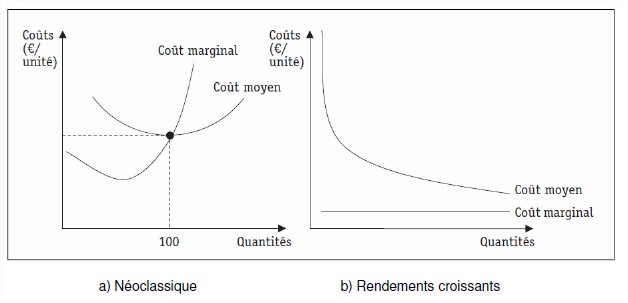
\includegraphics[scale=0.55]{2-7StructNat3.jpg}
					\caption{}\label{fig:struct_nat3}
				\end{figure}
			
				\begin{figure}[H]
					\centering
					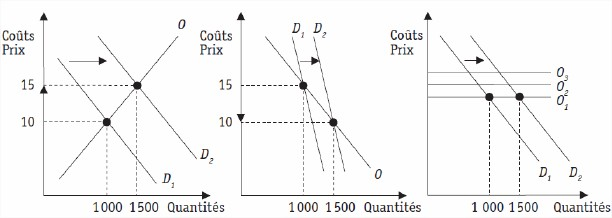
\includegraphics[scale=0.55]{2-7StructNat4.jpg}
					\caption{}\label{fig:struct_nat4}
				\end{figure}
			\end{itemize}
			\bigbreak
		
		
		
			\begin{mydef}[\textcolor{violet2}{\underline{Théorie de la régulation}}]
				L'état autorise les monopoles
				mais il existe une obligation de mettre un prix.
				Minimise la perte du surplus collectif.
			\end{mydef}
			\bigbreak



%%%%%%%%%%%%%%%%%%%%%%%%%%%%%%%%%%%%%%%%%%%%%%%%%%%%%%%%%%%%%%%%%%%%%%%%%%%%%%%%%

	\subsection{Monopole discriminant} % 2.8

		\subsubsection{Généralités}

			\begin{itemize}[label={\color{violet} \textbullet}]
			\item \textbf{En concurrence parfaite}:
			la firme n'a pas d'influence sur le prix.
			Elle se préoccupe seulement de son prix
			et choisit $q$ tel que $p = \cmarg$.
			\item Si il y a \textbf{pouvoir de marché} (ex.: monopole),
			la firme doit tenir compte des caractéristiques de la demande
			(ex.: par l'élasticité),
			même s'il n'y a qu'un seul prix pratiqué.
			\item \textbf{Stratégie plus sophistiquée}:
			tarifer \textcolor{blue}{des prix différents} pour des \textcolor{blue}{consommations différentes}.
			C'est-à-dire fixer un prix en fonction de la \textcolor{blue}{volonté à payer} du consommateur.
			\item \textbf{But}: capter tout ou une partie du $\surpluscons$
			et le transformer en profit supplémentaire pour la firme en monopole.
			\item \textbf{Outil} : discrimination par les prix.
			\end{itemize}
			\bigbreak



		\subsubsection{La capture du surplus du consommateur $\surpluscons$}


			\begin{minipage}{0.4\textwidth}
				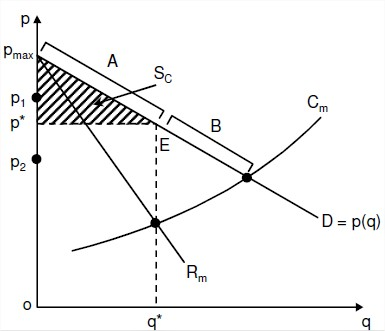
\includegraphics[width=\textwidth]{2-8CaptureSurplusC.jpg}
			\end{minipage}
			\begin{minipage}{0.55\textwidth}
				\begin{itemize}[label={\color{violet} \textbullet}]
					\item \textbf{Région} $\bm{A}$ : consommateurs prêts à payer $p_1$ tel que $p_1 > \popt$
					mais si ce prix est à $p_1$ (un seul prix pratiqué),
					des consommateurs ne consommeront plus (perte de consommateurs).
					\item \textbf{Région} $\bm{B}$:
					consommateurs prêts à payer $p_2$ tel que $\popt  > p_2 > \cmarg $,
					mais perte de profit sur d'autres consommations si un seul prix pratiqué.
					\bigbreak
					
					$\implies$ séparer les tarifications
					($p_1$ pour certains consommateurs de $\bm{A}$,
					$p_2 > \cmarg$ pour certains de $\bm{B}$).
				\end{itemize}
			\end{minipage}
			\bigbreak



		\subsubsection{Conclusions}

			\begin{itemize}[label={\color{violet} \textbullet}]
				\item Seul un monopoleur peut discriminer.
				\item La discrimination doit être pratiquée
				pour des raisons autres que des différences de coûts
				(coûts de production égaux).
				\item Pour qu'elle soit possible en pratique:
					\begin{itemize}[label={\color{Orchid} \textbullet}]
						\item les marchés doivent être cloisonnés
						(pas de revente possible);
						\item les clientèles doivent avoir des élasticités différentes.
					\end{itemize}
				\item Il y a 3 types de discrimination:
				\begin{itemize}[label={\color{Orchid} \textbullet}]
				\item \textbf{du 1\ieme{} degré}: pure;
				\item \textbf{du 2\ieme{} degré}: par blocs;
				\item \textbf{du 3\ieme{} degré}: séparation des marchés;
				\end{itemize}
			\end{itemize}
			\bigbreak

		\subsubsection{Discrimination du 1\ieme{} degré: pure}

			\begin{minipage}{0.4\textwidth}
				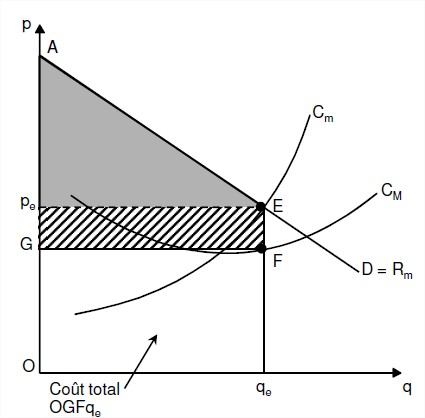
\includegraphics[scale=0.43]{2-8-1erDegre.jpg}
			\end{minipage}
			\begin{minipage}{0.53\textwidth}
				\begin{itemize}[label={\color{violet} \textbullet}]
					\item Pour un même bien,
					le monopole fixe un $p$ différent
					pour \textcolor{blue}{chaque unité} vendue.
					\item Le monopole doit donc connaître les fonctions de demande \textcolor{blue}{individuelles} de chaque consommateur.
					\item Quand on baisse le prix pour vendre une unité supplémentaire,
					on \textcolor{blue}{ne réduit pas} la recette sur les unités \textcolor{blue}{déjà vendues} à des $p$ supérieurs:
					chaque unité est vendue à un $p$ correspondant à la courbe de demande
					$\implies$ courbe $D \equiv \rmarg\,.$
					\item Production et vente optimales: $p = \cmarg $ (point $E$),
					identique à concurrence parfaite.
					\item Recette totale: $R = OAEq_{\textnormal{e}}\,.$
					\item Coût total de production: $q_{\textnormal{e}}\,.$
					\item Profit total: $\pcompt = AEFG\,.$
					\item $\surpluscons  = AEp_{\textnormal{e}}$ en concurrence parfaite
					et $\surpluscons = 0$ en monopole parfaitement discriminant.
					\item Paradoxalement, le monopole discriminant réalise un état \textcolor{blue}{Pareto-optimal}.
					\item \textbf{Mise en pratique}:
					difficile car nécessite la connaissance de la fonction de demande
					de chaque consommateur individuel.
				\end{itemize}
			\end{minipage}
			\bigbreak



		\subsubsection{Discrimination du 2\ieme{} degré: par blocs}



			\begin{minipage}{0.4\textwidth}
				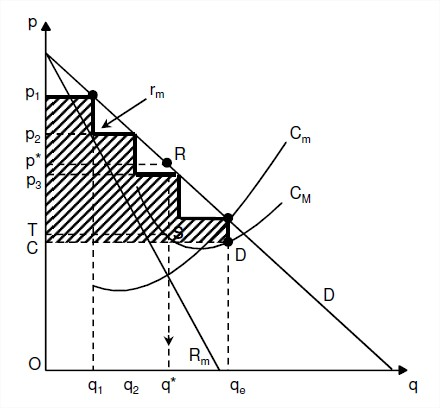
\includegraphics[scale=0.43]{2-8-2eDegre.jpg}
			\end{minipage}
			\begin{minipage}{0.53\textwidth}
				\begin{itemize}[label={\color{violet} \textbullet}]
					\item Vente à des prix différents,
					mais à prix identiques pour tous consommateurs achetant une \textcolor{blue}{même quantité} de biens.
					La discrimination par les prix est fonction des \textcolor{blue}{quantités achetées}
					et pas des \textcolor{blue}{individus}.
					\item $\rmarg  =$ fonction ``en escalier'' $r_{\textnormal{m}}\,.$
					\item $\max \pi$ implique de vendre tant que $r_{\textnormal{m}} > \cmarg\,.$
					\item \textbf{Coût unitaire}: $q_{\textnormal{e}} D = OC\,.$
					\item \textbf{Profit unitaire}: $\Delta (p1, p2,\dots \textnormal{ et }\cmoy)\,.$
					\item \textbf{Profit total}: $\pcompt$ (= surface hachurée) $> \pmon (\popt RST)\,.$
					\item \textbf{Mise en pratique}: pricing téléphonique, ristournes de quantités.
				\end{itemize}
			\end{minipage}
			\bigbreak



		\subsubsection{Discrimination du 3\ieme{} degré: séparation des marchés}


			\begin{myhyp}
				Le marché peut être scindé en (au moins) deux clientèles,
				avec des demandes et des élasticités-prix différentes.
			\end{myhyp}
			\bigbreak
			
			\begin{itemize}[label={\color{violet} \textbullet}]
				\item $D_1$, $R_{\textnormal{m},1}$ et $D_2$, $R_{\textnormal{m},2}$
				sont les fonctions caractéristiques de deux marchés
				qui ont été isolés et sont étanches (sinon ``reventes'').
				\item $D_{\textnormal{T}}$ et $R_{\textnormal{m,T}}$
				sont les fonctions caractéristiques
				correspondant à l’ensemble de ces deux marchés.
				\item $\cmarg$ le coût marginal de production,
				identique pour chacun des marchés.
			\end{itemize}
			
			\begin{figure}[H]
				\centering
				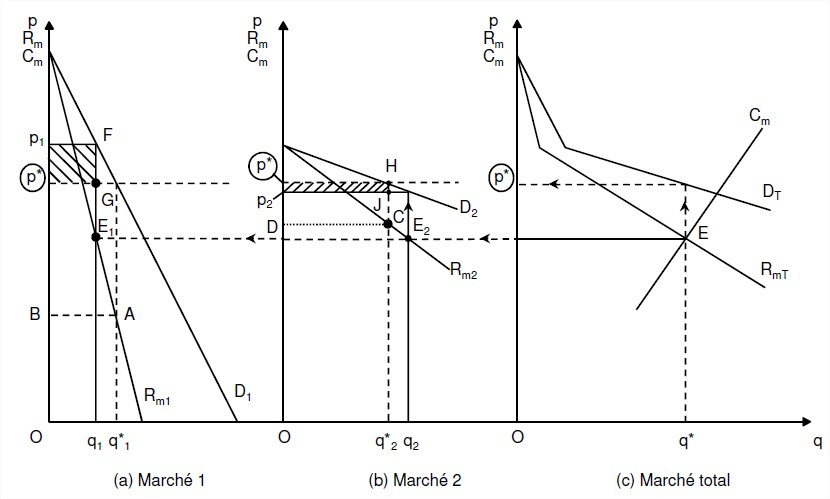
\includegraphics[scale=0.5]{2-8-3eDegre.jpg}
				\caption{}\label{fig:3rd_degree}
			\end{figure}
			
			
			\paragraph{Répartition des ventes entre les deux marchés (p. 98)}
			
			\begin{itemize}[label={\color{violet} \textbullet}]
				\item $R_{\textnormal{m},1} = R_{\textnormal{m},2} = \cmarg\,.$
				\item $\displaystyle\frac{p_1}{p_2} = \displaystyle\frac{1+\displaystyle\frac{1}{\elasticity_2}}{1+\displaystyle\frac{1}{\elasticity_1}} \implies \textnormal{si } \elasticity_1 > \elasticity_2 \implies p_2 < p_1\,.$
			\end{itemize}






%%%%%%%%%%%%%%%%%%%%%%%%%%%%%%%%%%%%%%%%%%%%%%%%%%%%%%%%%%%%%%%%%%%%%%%%%%%%%%%%%

	\subsection{La régulation des monopoles} % 2.9

		\textcolor{violet2}{\underline{But}} : annuler ou réduire la ``perte de Welfare''
		liée au comportement spontané du monopole. \bigbreak


		\subsubsection{Imposer la vente au coût marginal}



			\begin{minipage}{0.40\textwidth}
				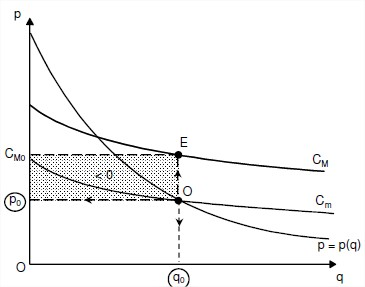
\includegraphics[scale=0.5]{2-9-1RegMon.jpg}
			\end{minipage}
			\begin{minipage}{0.55\textwidth}
				Mais si $\eta \: \textcolor{vert}{\nearrow} \implies \pcompt = p_0 q_0 - C_{\textnormal{M},0} \cdot q_0 = q_0 (p_0 - C_{\textnormal{M},0}) < 0\,.$
				\bigbreak
				$ p = \cmarg  \implies $ déficit d'exploitation systématique !
			\end{minipage}
			\bigbreak



		\subsubsection{Imposer la tarification au coût moyen}

			$\boxed{\eta \: \textcolor{red}{\searrow}}$
			\bigbreak

			\begin{minipage}{0.4\textwidth}
				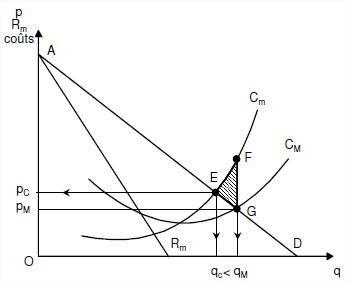
\includegraphics[scale=0.5]{2-9-2RegMon.jpg}
			\end{minipage}
			\begin{minipage}{0.5\textwidth}
				\begin{itemize}[label={\color{violet} \textbullet}]
					\item \textbf{Concurrence} : $p_{\textnormal{c}}$, $q_{\textnormal{c}}$ et $\surpluscons  = AEp_{\textnormal{c}}\,.$
					\item \textbf{Coût moyen} : $p_{\textnormal{M}} < p_{\textnormal{c}}$ et $q_{\textnormal{M}} > q_{\textnormal{c}}\,.$
					\item Mais perte de surplus $EFG$.
					(quantité $q_{\textnormal{c}} - q_{\textnormal{M}}$ produite à $\cmarg  >$ prix).
					\item Il y a surproduction
					et la tarification au $\cmoy$ n'est pas efficace.
				\end{itemize}
			\end{minipage}
			\bigbreak


			$\boxed{\eta \: \textcolor{vert}{\nearrow}}$
			\bigbreak

			\begin{minipage}{0.4\textwidth}
				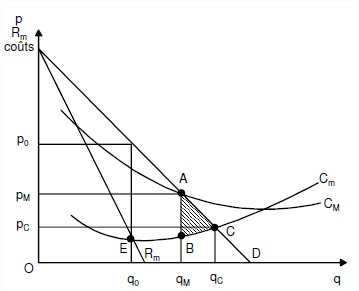
\includegraphics[scale=0.5]{2-9-2RegMon2.jpg}
			\end{minipage}
			\begin{minipage}{0.55\textwidth}
				\begin{itemize}[label={\color{violet} \textbullet}]
					\item \textbf{Concurrence} : $p_{\textnormal{c}}$, $q_{\textnormal{c}}\,.$
					\item \textbf{Monopole pur} : $p_0$, $q_0\,.$
					\item \textbf{Coût moyen} : $p_{\textnormal{M}}$, $q_{\textnormal{M}}\,.$
				\end{itemize}
				
				$\implies p=\cmoy$ est intermédiaire entre concurrence et monopole pur, mais il y a aussi perte de surplus $ABC$.

			\end{minipage}
			\bigbreak


		\subsubsection{Tarification de Ramsey-Boiteux (par segmentation du marché)}


			\begin{minipage}{0.4\textwidth}
				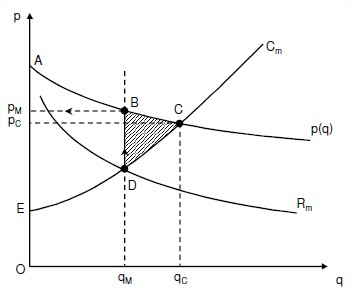
\includegraphics[scale=0.5]{2-9-3RegMon.jpg}
			\end{minipage}
		
			\begin{minipage}{0.55\textwidth}
				Si $p = \cmarg$: 
				surplus collectif max = $ACE$ (concurrence parfaite).
				
				Si $p \ne \cmarg $:
				surplus = $ABDE < ACE\,.$
				\bigbreak
				
				La surface $BDC$ représente
				la \textcolor{blue}{perte nette de Welfare}
				pour l'économie (producteurs et consommateurs).
			\end{minipage}
			\bigbreak


			\begin{minipage}{0.4\textwidth}
				\includegraphics[scale=0.5]{2-9-3RegMon2.jpg}
			\end{minipage}
			\begin{minipage}{0.55\textwidth}
				Introduction d'un prix par segment.
				\begin{itemize}[label={\color{violet} \textbullet}]
					\item $p_W = \cmarg$: Welfare, surplus maximum.
					\item Soit $p_{\mathsc{BUD}}$ : assure l'équilibre budgétaire
					du producteur, mais perte de Welfare !
	
					Perte = $MNW + KLW\,.$
					\item \textbf{Ramsey} : trouver $p_1$ et $p_2$
					tels que la perte de Welfare soit \textcolor{blue}{minimale},
					tout en respectant l'équilibre budgétaire:
					$YTW + ZSW < MNW + KLW\,.$
				\end{itemize}
			\end{minipage}
			\bigbreak



		\subsubsection{Récapitulatif}
		

			\begin{itemize}[label={\color{violet} \textbullet}]
				\item \textbf{Concurrence parfaite} : maximise le surplus collectif.
				\item \textbf{Monopole} :
				\begin{itemize}[label={\color{Orchid} \textbullet}]
					\item $p > p_{\textnormal{CP}}$ et $q < q_{\textnormal{CP}}\,.$
					\item n'arrive pas au max.
					\item parfois on ne sait pas faire mieux
					même si on n'est pas au max.
				\end{itemize}
				\item \textbf{Ramsey-Boiteux} :
				\begin{itemize}[label={\color{Orchid} \textbullet}]
					\item perte de surplus minimal.
					\item économiquement rentable.
					\item au plus un client est sensible au produit,
					au plus on lui fera payer.
					\item difficile à appliquer politiquement
					et on ne connaît pas l'élasticité de toutes les personnes.
				\end{itemize}
			\end{itemize}
			\bigbreak
			
			
		\subsubsection{Calcul analytique et généralisation à n segments (Lagrangien)}

			\[
			\boxed{\displaystyle\frac{p_i - \cmarg }{p_i} = \displaystyle\frac{-\lambda}{1 + \lambda} \cdot \displaystyle\frac{1}{\elasticity_i}} \quad \forall i= 1,\dots, n\,.
			\]
			
			Si les prix ne sont pas identiques : $\cmarg \to C_{\textnormal{m},i}\,.$

			\subsubsection{La régulation par contrats de ``price-caps''}

			\paragraph{Note} À lire p. 108.
			% TODO

		\subsubsection{La régulation par contrats de ``cost-plus''}

			\begin{itemize}[label={\color{violet} \textbullet}]
			\item \textbf{Principe}: permettre au monopole de tarifer
			à un prix $p > \cmarg$
			qui soit juste suffisant pour qu'il réalise un ``fair return''
			sur ses investissements.
			\item \textbf{Rentabilité sur capital}: $s = \displaystyle\frac{p\cdot q(K,L) - w L}{K}$ \quad ($w =$ taux de salaire pour le facteur travail).
			\item $\boxed{p \cdot \fdif{q}{L} = w}$ \quad Le monopole augmentera le recours au facteur travail
			jusqu'à ce que sa productivité marginale soit égale
			au taux de salaire (résultat classique).
			\item $\boxed{p \cdot \fdif{q}{K} < v}$ \quad La productivité marginale du capital mobilisé en régulation de cost-plus
			sera inférieure à celle sans régulation.
			
			$\implies$ Il y aura risque de ``surcapitalisation''
			et d'investissements excessifs.
			Besoin d'une implication forte du régulateur.
			\end{itemize}
		
%%%%%%%%%%%%%%%%%%%%%%%%%%%%%%%%%%%%%%%%%%%%%%%%%%%%%%%%%%%%%%%%%%%%
%%%%%%%%%%%%%%%%%%%%%%%%%%%%%%%%%%%%%%%%%%%%%%%%%%%%%%%%%%%%%%%%%%%%
%%%%%%%%%%%%%%%%%%%%%%%%%% Chapitre 3 %%%%%%%%%%%%%%%%%%%%%%%%%%%%%%
%%%%%%%%%%%%%%%%%%%%%%%%%%%%%%%%%%%%%%%%%%%%%%%%%%%%%%%%%%%%%%%%%%%%
%%%%%%%%%%%%%%%%%%%%%%%%%%%%%%%%%%%%%%%%%%%%%%%%%%%%%%%%%%%%%%%%%%%%



\section{La concurrence monopolistique}


%%%%%%%%%%%%%%%%%%%%%%%%%%%%%%%%%%%%%%%%%%%%%%%%%%%%%%%%%%%%%%%%%%%%%%%%%%%%%%%%%

	\subsection{Définition : situation hybride} % 3.1


		\begin{itemize}[label={\color{violet} \textbullet}]
			\item Nombreux producteurs (pas monopole).
			\item Différentiation $\implies$ assure un certain ``isolement''
			par rapport aux autres (choisit prix et quantité).
			\item Demande à la firme pas horizontale
			(c'est le cas en $\textnormal{CP}$)
			et pas la demande à toute la branche.
			\item 2 courbes de demande:
			\begin{itemize}[label={\color{Orchid} \textbullet}]
				\item $d$ = demande qui s'adresse à une entreprise $E$ donné
				si elle modifie son prix par rapport au prix $p_0$ en vigueur
				(les autres ne changeant rien).
				
				$p_0 \to p_1 \implies q_0 \to q_1'\,.$
				\item $D$ = demande qui s'adresse à l'entreprise
				si tous ses concurrents modifient simultanément
				et identiquement leurs prix.
				
				$p_0 \to p_1 \implies q_0 \to q_1\,.$
			\end{itemize}
		
			\begin{figure}[H]
				\centering
				\includegraphics[scale=0.7]{3-1Def.jpg}
				\caption{}\label{fig:sit_hybride}
			\end{figure}
		
			\item En $A$, $\elasticity_d > \elasticity_D\,.$
		\end{itemize}
		\bigbreak

		\renewcommand{\arraystretch}{1.5} % Espacement dans les cellules = 150% de l'espacement normal pour 1.5
		\begin{table}[H]
			\centering
			\begin{tabular}{lccc}
			\hline
			& Monopole & Concurrence monopolistique & Concurrence parfaite  \\
			Beaucoup d'acheteurs & + & + & +  \\
			Beaucoup de vendeurs & $-$ & + & +  \\
			Existence de substituts & $-$ & $\pm$ &  + \\
			Possibilité de fixer le prix & + & $\pm$ & $-$  \\
			\hline
			\end{tabular}
			\bigbreak
		\end{table}
		
		\begin{itemize}[label={\color{violet} \textbullet}]
			\item \textbf{Équilibre en CT} : $R_{\textnormal{m},1} = C_{\textnormal{m},1} \to q_1$ et $p_1$ avec $\ppur > 0\,.$
		
			Instable car concurrents entrent, attirés par $\ppur > 0\,.$
		\end{itemize}


%%%%%%%%%%%%%%%%%%%%%%%%%%%%%%%%%%%%%%%%%%%%%%%%%%%%%%%%%%%%%%%%%%%%%%%%%%%%%%%%%

	\subsection{Equilibre de LT en concurrence monopolistique} %3.2



		\begin{minipage}{0.4\textwidth}
			\includegraphics[scale=0.5]{3-2LT.jpg}
		\end{minipage}
		\begin{minipage}{0.55\textwidth}
			\begin{itemize}[label={\color{violet} \textbullet}]
				\item Arrivée de nouveaux conccurents
				$\implies$ demande à la firme baisse, vu l'existence de \textcolor{blue}{substituts} au produit
				($R_{\textnormal{M},1} \to R_{\textnormal{M},2}$).
				\item Ces entrées se font tant qu'un profit est possible,
				c'est-à-dire jusque $R_{\textnormal{M},2}  = \cmoy$
				(demande tangente au coût moyen).
				
				Point 2 = point de maximisation du profit.
			\end{itemize}
		\end{minipage}
		\bigbreak

		\textbf{Attention! Équilibre c. monop $\neq$ équilibre c. parfaite.}
		\begin{itemize}[label={\color{violet} \textbullet}]
			\item \textbf{CP} : $p_0 = \cmarg =$ minimum de $\cmoy\,.$
			\item \textbf{CM} : $\rmoy  = \cmoy\,, \rmarg = \cmarg$ et $p=\cmoy\,.$
			\item Il n'y a donc pas de maximisation du surplus global
			bien que le profit pur tende à disparaître.
			\item On peut montrer que la CM admet la CP comme cas limite si $n \to \infty\,.$
		\end{itemize}



%%%%%%%%%%%%%%%%%%%%%%%%%%%%%%%%%%%%%%%%%%%%%%%%%%%%%%%%%%%%%%%%%%%%
%%%%%%%%%%%%%%%%%%%%%%%%%%%%%%%%%%%%%%%%%%%%%%%%%%%%%%%%%%%%%%%%%%%%
%%%%%%%%%%%%%%%%%%%%%%%%%% Chapitre 4 %%%%%%%%%%%%%%%%%%%%%%%%%%%%%%
%%%%%%%%%%%%%%%%%%%%%%%%%%%%%%%%%%%%%%%%%%%%%%%%%%%%%%%%%%%%%%%%%%%%
%%%%%%%%%%%%%%%%%%%%%%%%%%%%%%%%%%%%%%%%%%%%%%%%%%%%%%%%%%%%%%%%%%%%



\section{Les marchés oligopolistiques}


%%%%%%%%%%%%%%%%%%%%%%%%%%%%%%%%%%%%%%%%%%%%%%%%%%%%%%%%%%%%%%%%%%%%%%%%%%%%%%%%%

	\subsection{Généralités et caractéristiques} % 4.1


		\begin{itemize}[label={\color{violet} \textbullet}]
			\item \textbf{Définition}: marchés où seul un \textcolor{blue}{petit nombre} de firmes
			assure toute (ou la plus grande partie) de la production.
			\item \textbf{Origines}: il existe des barrières à l'entrée,
			pas totales (comme en monopole)
			mais suffisantes pour empêcher l'atomicité de l'offre.
			\item \textbf{Institutionnelles}: les pouvoirs publics limitent l'entrée de nouveaux acteurs.
			\begin{itemize}[label={\color{Orchid} \textbullet}]
				\item Économies d'échelle (quantités).
				\item Économies de gamme (variétés).
				\item Différences de coût structurelles (brevets,\dots).
			\end{itemize}
			\item Situations, et donc management, plus complexes que :
			\begin{itemize}[label={\color{Orchid} \textbullet}]
				\item \textbf{Concurrence parfaite}: ici, les firmes ont une \textcolor{blue}{influence} sur le marché (comme en monopole).
				\item \textbf{Monopole} : mais elles ne sont \textcolor{blue}{pas seules} à fixer le prix (interactions entre elles).
			\end{itemize}
	
			\item \textbf{Concurrences} :
			\begin{itemize}[label={\color{Orchid} \textbullet}]
				\item \textbf{Parfaite} : relations ``anonymes''
				(personne ne se connaît),
				organisées par le seul intermédiaire des prix.
				\item \textbf{Oligopolistique} : relations stratégiques entre acteurs ``identifiés''.
			\end{itemize}
			\item Équilibres très différents en fonction du comportement des différents acteurs (firmes).
			\item Le produit peut être \textcolor{blue}{différencié} ou non.
			\item Petit nombre d'acteurs :
			\begin{itemize}[label={\color{Orchid} \textbullet}]
				\item ne signifie pas absence de concurrence\dots{};
				\item peut conduire à des ententes.
			\end{itemize}
		\end{itemize}
		\bigbreak


%%%%%%%%%%%%%%%%%%%%%%%%%%%%%%%%%%%%%%%%%%%%%%%%%%%%%%%%%%%%%%%%%%%%%%%%%%%%%%%%%

	\subsection{Nature de l'équilibre dans un marché oligopolistique} % 4.2


		\begin{itemize}[label={\color{violet} \textbullet}]
			\item \textbf{Rappels} :
			\begin{itemize}[label={\color{Orchid} \textbullet}]
				\item \textbf{Concurrence parfaite}: $p = \cmarg  \to q\,.$
				\item \textbf{Monopole}: $\rmarg  = \cmarg  \to q, p\,.$
				\item $p$, $q$, considérés comme donnés et $\pcompt$ maximisé en conséquence.
			\end{itemize}
		
			\item En \textbf{concurrence oligopolistique},
			on doit fixer $p$, $q$ en \textcolor{blue}{tenant compte explicitement} 
			du comportement des autres acteurs.
			
			\item \textbf{Principe}: chaque firme détermine $p$, $q$ en faisant aussi ``au mieux'',
			mais \textcolor{blue}{compte tenu} de ce que font ses compétiteurs,
			qui, eux aussi, font ``au mieux''.
			
			\item Tout dépendra donc des \textcolor{blue}{anticipations} que fera une firme sur le comportement des autres firmes.
		\end{itemize}
		\bigbreak
\end{document}
